% =====================================================================
% paper11_forecasting_baselines_v67.tex
% Forecasting against naive benchmarks: a scored test of process-based
% modules on Northern cod and the Edwards Aquifer
% Author: Amin Abaee (Independent Researcher, Tehran, Iran)
%
% Lineage: paper11_forecasting_baselines_v66 (two-part article: Part I cod =
% paperE1 v60 + related-work subsection; Part II Edwards J-17 = paper11b v2;
% cross-system conclusion) -> v67 (this file): one research article with a
% shared design section, two system sections, a cross-system synthesis that
% states and proves the increment decomposition (Proposition 2) and the
% horizon-crossover criterion (Remark 2), a merged related-work section and a
% combined Supplementary Information. The cod half carries the research-article
% restructuring of paperE1_cod_forecast_ladder_v69 (period decomposition,
% identification result, operating characteristics); that v69 file was built
% from the stale v59/v60 base and is superseded by this edition.
% No archived score was changed. New computations in this edition (the
% horizon profile h = 1..5 of the two baselines on all three series, the
% autocorrelations used by Proposition 2 and Fig. 7) are reproduced by
% work/make_fig_mechanism.py and work/horizon_profile.py from the registered
% data files (SI S16, S23).
% Target: Environmental Modelling & Software (elsarticle, author-year).
% Compiles with pdfLaTeX / XeLaTeX / LuaLaTeX / tectonic.
% =====================================================================
\documentclass[preprint,11pt,authoryear]{elsarticle}

\usepackage{amsmath,amssymb,amsthm}
\usepackage{booktabs}
\usepackage{array}
\usepackage{tabularx}
\usepackage{multirow}
\usepackage{graphicx}
\graphicspath{{./}{figs/}{paper11_forecasting_baselines_v67_src/figs/}}
\usepackage{enumitem}
\usepackage{placeins}
\renewcommand{\topfraction}{0.9}
\renewcommand{\bottomfraction}{0.7}
\renewcommand{\textfraction}{0.07}
\renewcommand{\floatpagefraction}{0.75}
\usepackage[colorlinks=true,urlcolor=blue,linkcolor=blue,citecolor=blue]{hyperref}
\emergencystretch=3em
\setlength{\tolerance}{2000}

\newtheorem{proposition}{Proposition}
\theoremstyle{definition}
\newtheorem{definition}{Definition}
\theoremstyle{remark}
\newtheorem{remark}{Remark}

\newcommand{\kt}{\,\mathrm{kt}}
\newcommand{\ft}{\,\mathrm{ft}}
\newcommand{\Blim}{B_{\mathrm{lim}}}
\newcommand{\Spos}[1]{\left[#1\right]_{+}}
\newcommand{\RMSE}{\mathrm{RMSE}}
\newcommand{\MAE}{\mathrm{MAE}}
\newcommand{\MSE}{\mathrm{MSE}}
\newcommand{\pers}{\mathrm{persist}}
\newcommand{\sA}{\mathfrak{s}}
\newcommand{\E}{\mathbb{E}}
\newcolumntype{Y}{>{\centering\arraybackslash}X}
\newcolumntype{L}{>{\raggedright\arraybackslash}X}

\journal{Environmental Modelling \& Software}

\begin{document}

\begin{frontmatter}

\title{Forecasting against naive benchmarks: a scored test of process-based modules on Northern cod and the Edwards Aquifer}

\author[1]{Amin Abaee\corref{cor1}}
\ead{amin_abaee@ut.ac.ir}
\cortext[cor1]{Corresponding author. ORCID: 0000-0002-0019-1842.}
\affiliation[1]{organization={Independent Researcher}, city={Tehran}, country={Iran}}

\begin{abstract}
Adding a mechanism to a forecasting model is a claim that the mechanism helps to predict the system, and the claim can be scored against the forecast that nothing changes. We report one such test on two unrelated systems: a five-module surplus-production ladder on the spawning-stock biomass of Northern cod (\emph{Gadus morhua}, NAFO 2J3KL; the 1983--2015 NCAM and the 1954--2024 xteNCAM series) and a one-pool water-balance ladder on annual-mean head at the Edwards Aquifer index well J-17 (1934--2023). Both ladders are scored by rolling-origin RMSE against last-value persistence and the training mean, each under its own disclosed retention protocol, and the two systems' scores are never pooled. No structural module is retained on either system. On cod, persistence has one-year RMSE 98\,kt against 115--196\,kt for the modules (84 against 119--206\,kt on the longer series); the deficit is carried by the 1991--1995 collapse, which no member of the class can reproduce at the recorded catch, and under known truth the rule retains a true autonomous module in 97\% of replicates, so the verdict is a property of the series rather than of the test. On J-17, a balance that persists last year's recharge loses to persistence (14.70 against 13.23\,ft) because annual recharge is near-white ($r=0.17$) while the head increment tracks it ($r=0.74$); a univariate AR(1) is retained by the aquifer protocol by a 0.39-ft margin whose bootstrap interval covers zero; the same map given the year's realised fluxes nowcasts at 7.55\,ft; and the training mean beats persistence from two years ahead. An elementary decomposition explains both outcomes: a one-step structural forecaster gains on persistence only through what its mechanism fits of the realised increment and loses whatever its substituted driver fails to persist, the persisted-driver term being negative whenever the driver's lag-one autocorrelation is below one half; and the training mean overtakes persistence at the horizon at which the predictand's autocorrelation falls below one half. The two systems fail on the two different terms of that decomposition, which is why one test and two protocols yield one lesson: mechanistic fidelity is a hypothesis about accuracy, to be scored rather than assumed.
\end{abstract}

\begin{keyword}
forecast evaluation \sep persistence benchmark \sep rolling-origin scoring \sep model retention \sep surplus production \sep Northern cod \sep water balance \sep Edwards Aquifer \sep Diebold--Mariano test
\end{keyword}

\end{frontmatter}

\section{Introduction}\label{sec:intro}

A process-based forecasting model earns its structure by predicting better than a model without it. The forecasting literature has made that requirement operational: a candidate is held to beat a naive benchmark, usually last-value persistence and the training mean, out of sample at the horizons that matter \citep{Makridakis2000,HyndmanKoehler2006,HyndmanAthanasopoulos2021}; the evaluation is run on a rolling origin so that each forecast uses only what was available when it would have been issued \citep{Tashman2000,Bergmeir2012}; and differences in accuracy are tested rather than eyeballed \citep{Diebold1995,Harvey1997,Diebold2015}. Applied to environmental systems these standards have produced a consistent and uncomfortable result. Simple time-series models forecast fish populations about as well as complex ones \citep{Ward2014}, model-free methods have outperformed the mechanistic models that generated the data when the mechanism is unstable \citep{Perretti2013}, and in the largest forecasting competitions the sophisticated entries have rarely beaten the simple statistical ones \citep{Makridakis2000,Makridakis2018}. Yet in the applied literatures that build process models for management, the added mechanism is still widely treated as a reason to prefer the model, and the benchmark comparison, where it is made at all, is seldom made under a rule fixed before the scores are seen.

This paper reports one scored test on two systems that share nothing but the question. The first is the spawning-stock biomass (SSB) of Northern cod (\emph{Gadus morhua}) in NAFO Divisions 2J3KL, the archetype of a fishery collapse \citep{Hutchings1994,Myers1997} and of a contested recovery \citep{RoseRowe2015,Rose2026}, on which two retrospective assessment series exist: the 1983--2015 NCAM series \citep{Cadigan2016,DFO2016} and the 1954--2024 xteNCAM series of the 2024 framework revision \citep{Regular2025}. The candidate structure is a ladder of nested surplus-production forecasters \citep{Schaefer1954,Pella1969}: an autonomous module driven by the training-mean catch, a depensatory variant, a stock-flow module that receives the realised catch along the horizon, an autoregressive-residual correction and a lagged-start variant. The second system is the annual-mean head of the Edwards (Balcones Fault Zone) Aquifer at index well J-17, San Antonio, Texas, 1934--2023, one of the longest managed groundwater records in North America, on which drought-stage declarations and springflow protection key \citep{EAA2024}. The candidate structure is a one-pool water balance in which the head increment is a weighted sum of recharge and pumpage plus a linear drain, with residual, delay and climate-informed variants, scored beside a univariate AR(1). Both ladders are deliberately simple, and both are of a kind that practitioners use and defend on mechanistic grounds; neither is a straw man, and neither is a state-of-the-art model. The question asked of each is the same: does any structural step lower the out-of-sample error of the predictand that management actually uses, relative to persistence and to the step below it, at the horizons at which advice is issued?

The two systems are evaluated by one scoring core and two retention protocols, and the distinction matters for how the results should be read. The scoring core, shared, is rolling-origin RMSE on the predictand at one- and five-year horizons against origin-matched persistence and training-mean baselines, with Diebold--Mariano statistics and moving-block bootstrap intervals on every load-bearing margin. The retention protocols are system-specific and are reported as they were applied: on cod, a module is kept only if it beats both its comparator and persistence by more than a 5\% band at both horizons; on the aquifer, a module is kept if it beats persistence and the next-simpler causal model on the point one-year RMSE, with no band. Each protocol had its scoring core coded before the first pass and had elements completed after scores were seen (the cod tie band and non-nested comparator declarations; the aquifer class clause and climate-rung comparator), and each completion is disclosed with its effect on the verdict, which in every case is nil. The design is a fixed computational protocol with a recorded pass order, not a prospective registration, and we do not call it one. The two systems' scores are never pooled, no retention verdict is transferred between them, and each system also reports what the test could have detected: by simulation under known truth on cod, and by the oracle and nowcast diagnostics on the aquifer.

The result is uniform and, we argue, instructive beyond the two systems. No structural module is retained on either. On cod the modules' one-year RMSE is 17--100\% above persistence on the first series and 42--144\% above it on the second; the pooled deficit is carried by the 1991--1995 collapse, which no member of the surplus-production class can reproduce at the recorded catch because those years removed more biomass than the catch record accounts for; the autonomous modules forecast the numerical floor at every post-collapse origin because training-mean catch exceeds the production of a depleted stock; and under known truth the rule retains a true autonomous module in 97\% of replicates, so its non-retention is evidence about the series. On J-17 the balance that persists last year's recharge loses to persistence at one year (14.70 against 13.23\,ft) because annual recharge is near-white ($r(R_t,R_{t-1})=0.17$) while the head increment is strongly coupled to same-year recharge ($r(\Delta H_t,R_t)=0.74$); the univariate AR(1) is retained by the aquifer protocol by 0.39\,ft, a margin whose bootstrap interval covers zero and which reverses at five years; the same balance given the realised fluxes nowcasts the year at 7.55\,ft; climate predictors known at the origin recover at most 0.13\,ft of the gap; and the training mean beats persistence at every horizon from two years. The two failures have different proximate causes, a class failure in the fishery and a driver-persistence failure in the aquifer, and part of the contribution of this paper is to show that they are the two terms of one elementary decomposition rather than two unrelated anecdotes.

Three things are new relative to the two single-system studies from which this article descends and to their earlier two-part combination. First, the cross-system reading is formalised. Proposition~\ref{prop:increment} decomposes the one-step mean squared error of any forecaster of the form ``last value plus a mechanism evaluated at a substituted driver'' relative to persistence into a term that depends only on what the mechanism fits of the realised increment and a term that depends only on how the substituted driver fails to persist; the second term is negative whenever the driver's lag-one autocorrelation is below one half, and the climatological-flux forecaster never loses to persistence. Remark~\ref{rem:crossover} states the companion criterion for the baselines: under stationarity the training mean overtakes persistence at the horizon at which the predictand's autocorrelation falls below one half. On J-17 both statements are quantitatively borne out; on cod the increment decomposition locates the failure in the mechanism term and the crossover criterion fails, as it should for a non-stationary series. An earlier combination of the two studies attributed the cod failure to a ``weakly autocorrelated'' surplus production; the apparent net production of the assessed series has lag-one autocorrelation 0.71--0.91, and the attribution is withdrawn here in favour of the class argument of Proposition~\ref{prop:repeller}. Second, the aquifer results are reported under both protocols, so that the reader sees that the AR(1) is retained under the aquifer's point rule and not under the cod band-and-two-horizon rule, and sees why. Third, the horizon profile of the two baselines is computed at every horizon from one to five years on all three series from the registered data, which turns the five-year climatology result into a crossover with a predicted location.

The paper is organised as a single argument. Section~\ref{sec:design} sets out the shared scoring core, the two protocols and the operating-characteristic designs. Sections~\ref{sec:cod} and \ref{sec:edwards} report the two systems, each with its data, ladder, verdict and diagnostics. Section~\ref{sec:synthesis} states and verifies the decomposition and the crossover criterion, and tabulates what transfers between the systems and what does not. Section~\ref{sec:related} positions the work in the forecast-evaluation, fisheries and groundwater literatures. Section~\ref{sec:discussion} discusses the limits of the findings and Section~\ref{sec:conclusions} concludes. Proofs are in \ref{app:proofs}. Material that supports but does not carry the argument (pass orders, origin sets, full test grids, fitted parameters, fixed-window and variant passes, the simulation design, the aquifer service-series and pumpage layers, the horizon profiles, the vintage and suspension records and the verification record) is in the Supplementary Information (SI), whose sections are cited as S1--S23.
\section{One scoring core, two retention protocols}\label{sec:design}

\subsection{The object scored}\label{sec:object}

In both systems the predictand is the quantity that management reads, not a fitted index of it: assessed SSB in kilotonnes for cod, and the calendar-year mean of daily-high J-17 elevation in feet above mean sea level for the aquifer. Each candidate forecaster is a \emph{module} on a \emph{ladder}: a forward-ordered set of models in which each rung adds one structural element to the rung below, so that the contribution of each element can be isolated by comparing a module with its comparator (the next-simpler module) and not only with a naive benchmark. Two baselines are scored on every origin set: last-value persistence, $\hat y_{t+h}=y_t$, and the training mean, $\hat y_{t+h}=\bar y_{1:t}$ (``climatology''). Baselines are always computed on exactly the origin set used for the modules at that horizon, so that every comparison is origin-matched.

\subsection{Scores, origins and horizons}\label{sec:scores}

The primary score is the root mean squared error of the point forecast in the predictand's own units; mean absolute error is reported alongside, and indicator (Brier) scores for the management threshold are secondary and play no part in retention (SI S7, S19). Two evaluation designs are used in both systems. \emph{Fixed windows} fit once on a training window and forecast the following test window as a path; they are diagnostic, and show how a module behaves across an event (a collapse, a recovery, a drought of record) whole. The \emph{rolling-origin} design \citep{Tashman2000} is the one the retention protocols are applied to: at every origin $t$ from the first admissible year to the last that leaves $h$ target years, each module is refitted on the data through $t$ and a forecast of $y_{t+h}$ is scored; the errors are pooled across origins. Horizons are $h=1$ and $h=5$ years in both systems (the horizons at which annual advice and multi-year planning are issued); the horizon profile $h=1,\dots,5$ of the two baselines is added in Section~\ref{sec:synthesis}. Minimum training lengths are 8 years (cod, Specification A), 12 years (cod, Specification B) and 15 years (J-17), giving origin counts of 25/21, 59/55 and 75/71 at $h=1$/$h=5$ (SI S2, S16).

\subsection{The information set at the origin}\label{sec:info}

A forecast issued at origin $t$ for target $t+h$ may use only quantities dated $t$ or earlier, with declared exceptions that are the structural claim under test. On cod, the stock-flow modules receive the realised catch $C_{t+1},\dots,C_{t+h}$ along the horizon: the forecast is conditional on removals, the form in which surplus-production projections are issued (``if removals are $C$, biomass will be $S$''), and it gives those modules information the baselines never see, so that the persistence benchmark is conservative for them. The autonomous cod modules hold catch at its training mean. On J-17 the causal modules must substitute something for the unknown year-$(t+1)$ fluxes: last year's values (M2), the training-mean fluxes (M2m), or a one-step recharge forecast from climate indices known in year $t$ (climate-informed variants); an \emph{oracle} that receives the realised fluxes is scored as a diagnostic and excluded from retention. The contrast between the two systems is deliberate. On cod the driver (catch) is supplied; on J-17 the driver (recharge) must be forecast. Section~\ref{sec:synthesis} shows that this difference decides which term of the error decomposition each system fails on.

\subsection{The two retention protocols}\label{sec:protocols}

Each system is judged by the protocol under which it was scored. Both protocols share a scoring core, coded before the first scoring pass of the respective system and applied unchanged: compare the module's rolling-origin RMSE with origin-matched persistence and with its comparator, on declared windows and origin sets. They differ in the decision predicate.

\begin{center}
\fbox{\parbox{0.95\textwidth}{\small
\textbf{Protocol C (cod).} A module $M$ with comparator $M'$ is \emph{retained} on a specification if and only if, in the rolling-origin design,
\begin{enumerate}[label=(C\arabic*),leftmargin=3em,itemsep=1pt]
\item $\RMSE(M) < 0.95\,\RMSE(M')$ at both $h=1$ and $h=5$ (comparator hurdle; vacuous for the first rung), and
\item $\RMSE(M) < 0.95\,\RMSE(\pers)$ at both $h=1$ and $h=5$ (persistence hurdle), and
\item both hold on the same specification; a win on Specification A does not carry to B or conversely.
\end{enumerate}
The 5\% band treats differences within it as ties.

\medskip
\textbf{Protocol E (Edwards).} A causal module $M$ is \emph{retained} if and only if, at $h=1$ on the point rolling-origin RMSE,
\begin{enumerate}[label=(E\arabic*),leftmargin=3em,itemsep=1pt]
\item $\RMSE(M) < \RMSE(\pers)$, and
\item $\RMSE(M) < \RMSE(M_{\text{next-simpler causal}})$.
\end{enumerate}
No tie tolerance and no minimum margin is imposed; diagnostic oracles and the service series are excluded from retention.}}
\end{center}

Both protocols are decision rules on point estimates; the uncertainty layer of Section~\ref{sec:uncertainty} describes their margins but is not part of either. Protocol C is the stricter, and when the J-17 scores are restated under it no module is retained (Section~\ref{sec:edw_verdict}); Protocol E retains the aquifer's AR(1). We report both, because the purpose is not to make the two systems agree but to show what each rule does with the same scores.

\paragraph{What was completed after scores were seen.} Neither protocol was prospectively registered, and the honest description is a fixed computational protocol with disclosed completions. On cod, the 5\% band and the comparator declarations for the non-nested modules were formalised after the first pass had been scored; neither decides any outcome, the smallest pooled deficit being 17.1\% (SI S1 records the pass order). On J-17, the frozen protocol documents (dated 2026-08-25) contain the retention predicate verbatim, but three elements sit outside it and are recorded as deviations: a \emph{class clause} by which the climatological-flux map M2m, which satisfies (E1) and (E2), is listed and then declined because under constant fluxes it reduces to the AR(1) function class; the declaration of the retained AR(1), rather than the declined M2m, as the comparator for the climate-informed rung; and a struck direction-of-change score for which no value is reported (SI S15). The class clause is the one completion with a visible consequence, and Section~\ref{sec:edw_verdict} reports the verdict with and without it.

\paragraph{No pooling.} The two systems are never pooled, concatenated or averaged; nor are the two cod specifications, whose 1983--2015 overlap differs by 126\,kt RMSE between vintages. Every number in this paper belongs to one series under one protocol, and the cross-system statements of Section~\ref{sec:synthesis} are statements about mechanisms, not about pooled skill.

\subsection{Uncertainty of the margins}\label{sec:uncertainty}

For every load-bearing module--benchmark pair the per-origin squared-error differences $d_t = e^2_{M,t}-e^2_{B,t}$ are summarised by the Diebold--Mariano statistic \citep{Diebold1995} with an autocorrelation-consistent variance truncated at lag $h-1$, the form appropriate to $h$-step errors, reported as a $z$-score without the small-sample correction of \citet{Harvey1997}. It is not the primary uncertainty statement: samples are small, the loss differences are heavy-tailed because a few event-year errors dominate the sums of squares, and the asymptotic reference overstates significance in that setting \citep{Diebold2015}. The primary statement is a paired moving-block bootstrap \citep{Kunsch1989} of the RMSE gap, with the same block indices applied to both loss series; block length $\max(h,3)$ and 20\,000 replicates on cod, block length 8 and 10\,000 replicates on J-17 with an independent second implementation at block length $h$ and 20\,000 replicates (SI S3, S18). Block-length sensitivity is reported in both systems and no conclusion depends on it.

\subsection{What the test could have seen}\label{sec:power}

A non-retention can mean that the structure is absent or that the test could not see it, and the two systems supply the distinction by different means. On cod, seven data-generating processes were simulated at the fitted parameters of the fixed windows (200 replicates each, two process-noise levels): the autonomous truth at collapse- and recovery-window parameters, the stock-flow truth, the depensatory truth, a persistence-true null, and two truths outside the class; each replicate was scored by Protocol C, with pre-declared bars of power $\ge 0.80$ and false retention $\le 0.10$ (SI S8). On J-17 the corresponding evidence is the oracle: the same one-pool map, given the realised fluxes of the target year, scores 7.55\,ft against persistence's 13.23\,ft, so the mechanism is demonstrably able to explain the increment when its driver is known, and the forecasting failure is located in the driver rather than in the map (Section~\ref{sec:edw_mech}). The two designs answer the same question, whether the instrument is capable of a positive result, and in both systems the answer is yes.
\FloatBarrier
\section{System I: Northern cod, NAFO 2J3KL}\label{sec:cod}

\subsection{Two assessment series, kept separate}\label{sec:specs}

The predictand is spawning-stock biomass in kilotonnes. Two retrospective series are used, each as a separate specification with its own catch record, threshold, test windows and origin set (Table~\ref{tab:specs}, Fig.~\ref{fig:series}). They are never pooled, concatenated or spliced: the two assessment models differ in structure, natural-mortality treatment and catch handling, and their overlap for 1983--2015 differs by 126\,kt RMSE with the NCAM series higher on average by 58\,kt, so a forecast scored across a junction would be scored partly on a vintage change.

\textbf{Specification A} is the NCAM retrospective of \citet{Cadigan2016} in the M-shift formulation, as tabulated for the 2016 assessment \citep[Table A2]{DFO2016}: 33 annual SSB values for 1983--2015. Its limit reference point (LRP) is the 1983--1989 mean, $884.6\kt$ \citep{DFO2009,DFO2016}; the 2015 value, $298.65\kt$, is 33.8\% of it. Two catch records are used in two separate passes. The primary pass uses a coarse regime schedule declared before any model was fitted: 240\,kt per year through 1991, 120\,kt in 1992 and 5\,kt from 1993 onward, a stylised representation of the pre-moratorium fishery, the partial moratorium year and the residual removals thereafter. The second pass replaces it with the annual landings series of \citet{Schijns2021}, which matches the reported 2015 landings exactly but, like all landings series for this stock, remains below total removals. \textbf{Specification B} is the xteNCAM retrospective of the 2024 framework revision \citep[Table 17]{Regular2025}: 71 annual SSB values for 1954--2024 with published 95\% intervals. Its threshold is $\Blim = 276\kt$, defined as 40\% of $B_{\mathrm{MSY}}$ \citep{DFO2024a}. Catch is the official 2J3KL landings record \citep[Table 1]{Regular2025} for 1954--2023, with 2024 carried from 2023.

Both specifications use a single retrospective vintage throughout: every forecast is scored against the value the same assessment later assigned to the target year, not against the value a contemporaneous assessment would have published. This is standard in hindcast evaluation and it favours the models slightly, since retrospective revisions have smoothed the series the models are fitted to; the size of the effect is bounded in Section~\ref{sec:verdict}. Parameters are refitted at every origin on the expanding training window. The thresholds enter only the secondary indicator score (SI S7), never a forecast.

\begin{table}[!htb]
\centering\small
\caption{The two cod specifications. Each is scored on its own; nothing is pooled across the two. Rolling-origin counts are for the ladder modules; the baselines are evaluated on the identical origin sets.}
\label{tab:specs}
\begin{tabularx}{\textwidth}{@{}>{\raggedright\arraybackslash}p{0.2\textwidth}LL@{}}
\toprule
 & Specification A & Specification B \\
\midrule
Assessment & NCAM, M-shift formulation \citep{Cadigan2016}; \citet[Table A2]{DFO2016} & xteNCAM, revised framework; \citet[Table 17]{Regular2025} \\
Years & 1983--2015 (33 states, 32 transitions) & 1954--2024 (71 states, 70 transitions) \\
Predictand & SSB (kt), one retrospective vintage & SSB (kt), one retrospective vintage, with published 95\% interval \\
Catch & primary pass: coarse regime 240/120/5\,kt (through 1991 / 1992 / from 1993); second pass: annual landings \citep{Schijns2021} & annual landings 1954--2023 \citep[Table 1]{Regular2025}, 2024 carried from 2023 \\
Threshold (secondary score only) & LRP $=$ 1983--1989 mean $= 884.6\kt$ & $\Blim = 276\kt$ (40\% $B_{\mathrm{MSY}}$) \\
Fixed windows & collapse: train 1983--1990, test 1991--1995; recovery: train 1995--2007, test 2008--2015 & collapse: train 1954--1989, test 1990--1995; recovery stall: train 1995--2012, test 2013--2024 \\
Rolling origins & minimum 8 training years; origins 1990--2014 ($n=25$, $h=1$) and 1990--2010 ($n=21$, $h=5$) & minimum 12 training years; origins 1965--2023 ($n=59$) and 1965--2019 ($n=55$) \\
Last common year & 2015: $298.65\kt$ (33.8\% of LRP) & 2015: $273\kt$ (0.99 $\Blim$) \\
\bottomrule
\end{tabularx}
\end{table}

\begin{figure}[!htb]
\centering
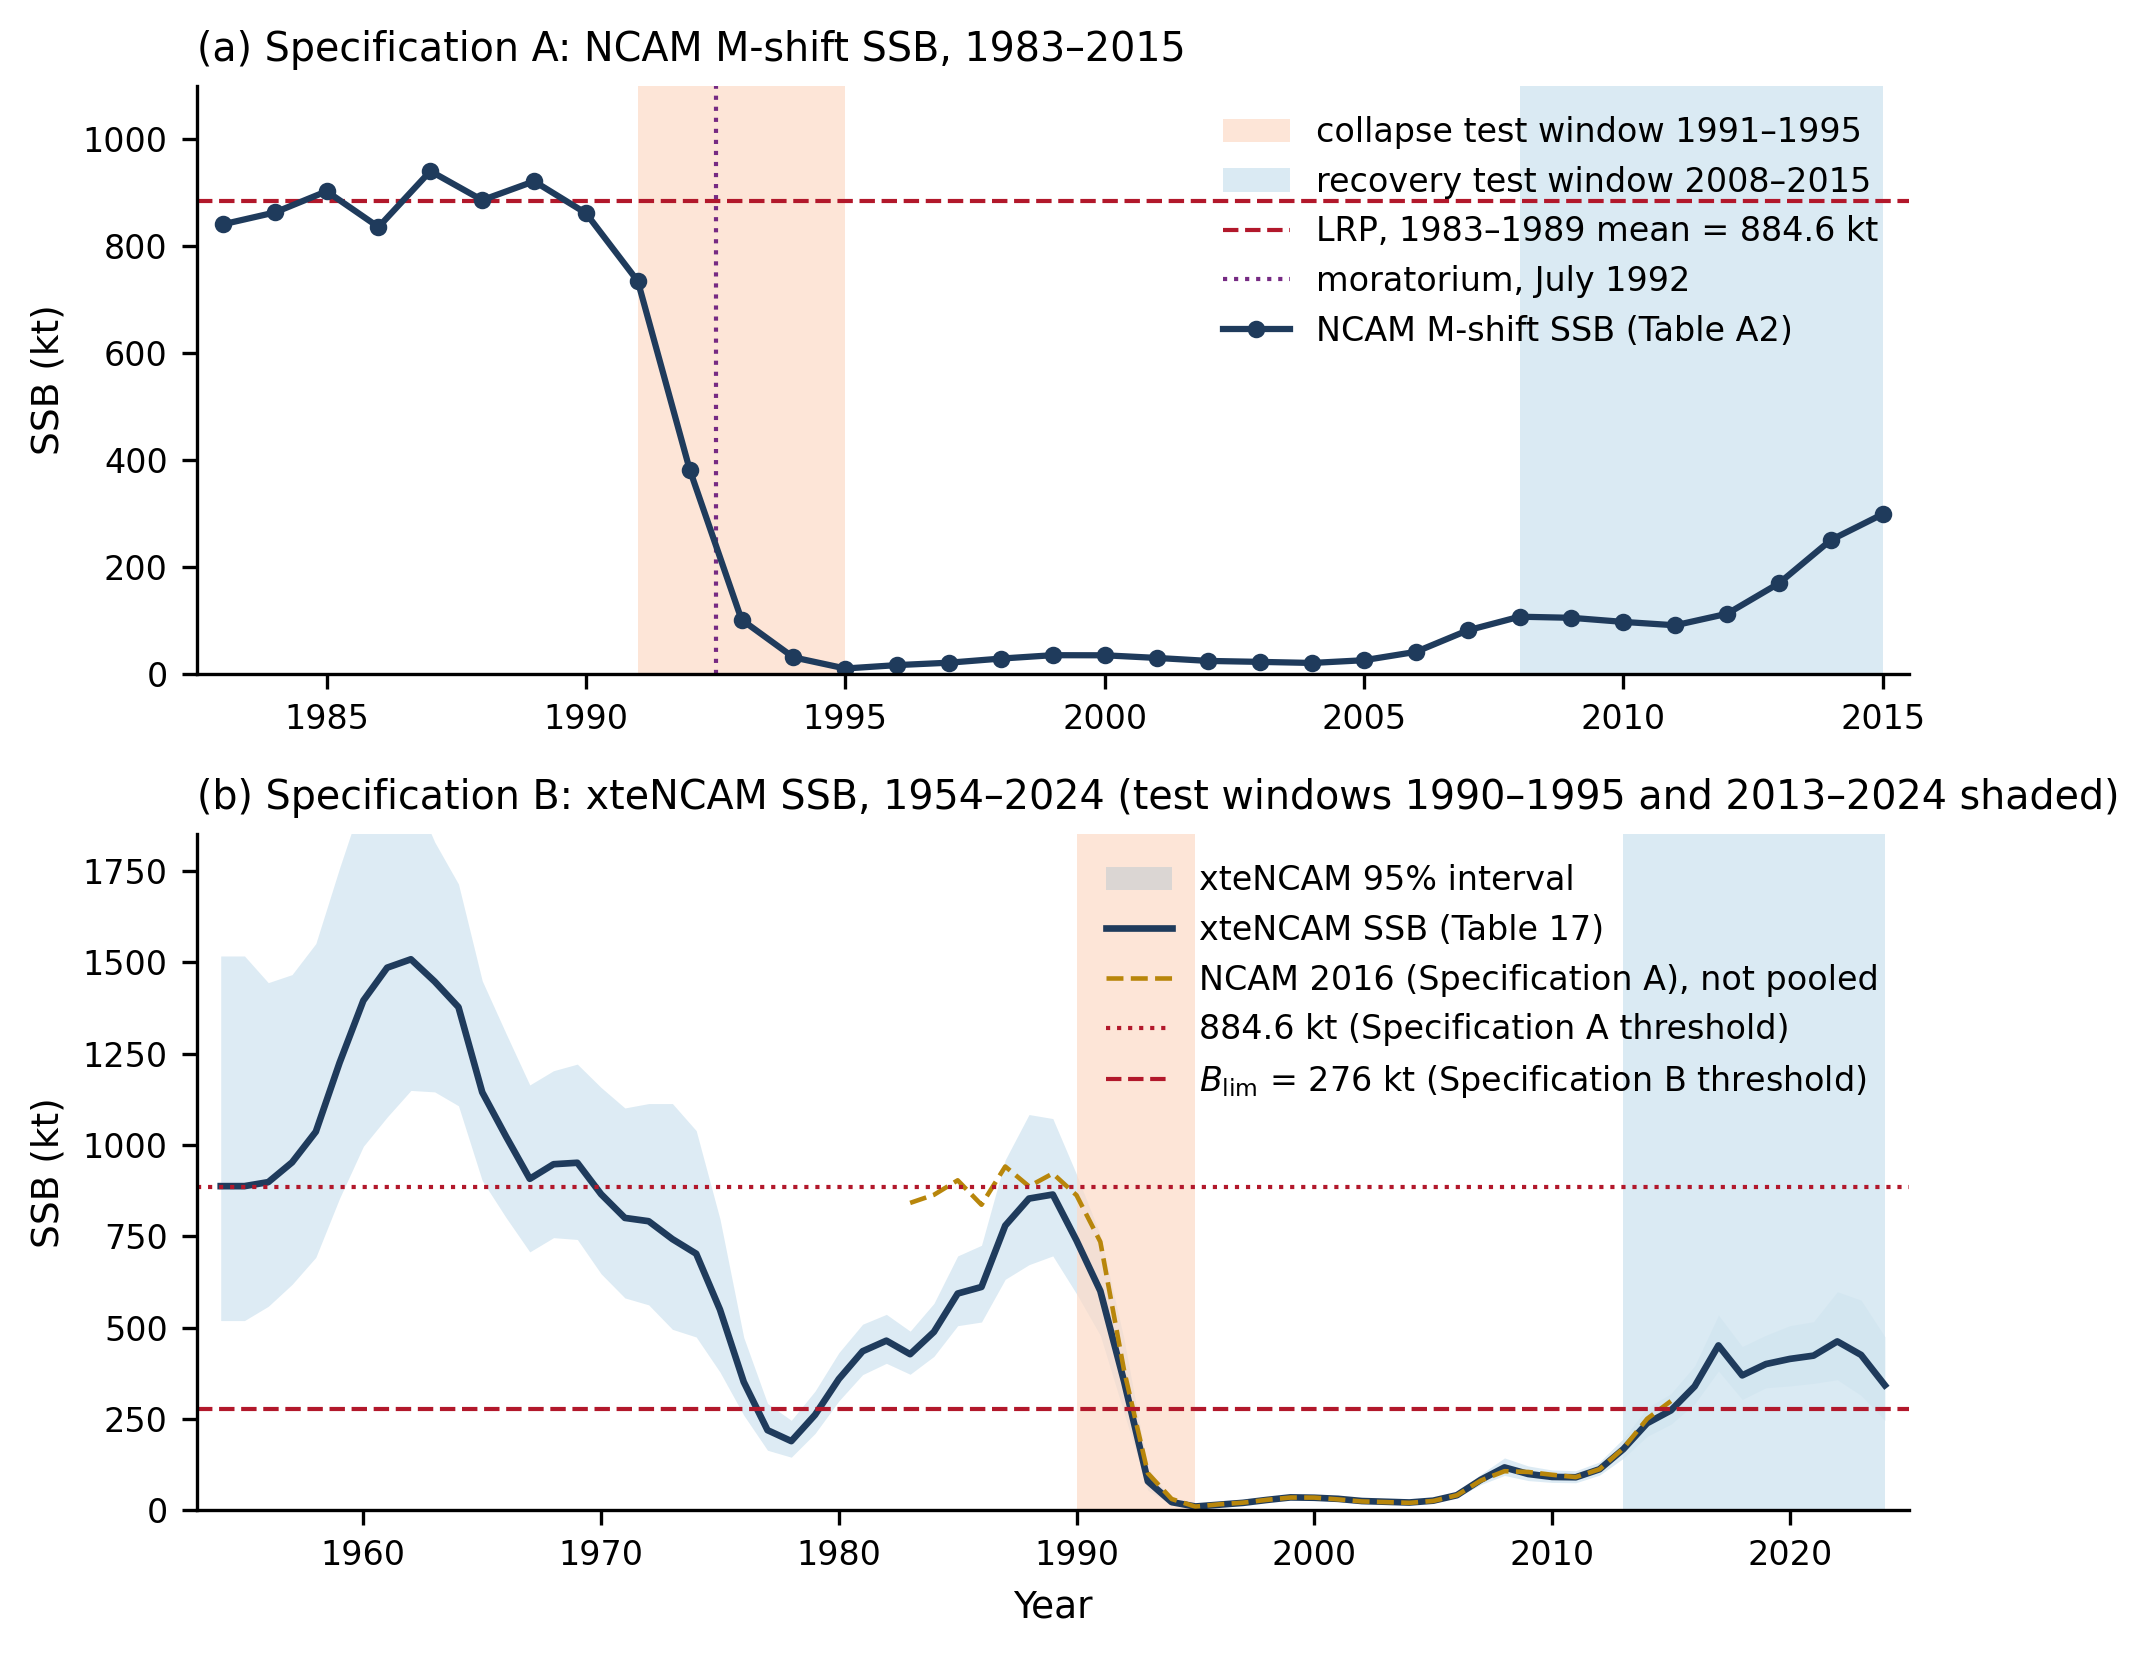
\includegraphics[width=\textwidth]{fig1_series}
\caption{The two SSB series on which the cod ladder is scored. (a) Specification A: NCAM M-shift SSB 1983--2015, with the LRP (1983--1989 mean, 884.6\,kt), the July 1992 moratorium and the two fixed test windows. (b) Specification B: xteNCAM SSB 1954--2024 with its published 95\% interval, $\Blim = 276\kt$, and the NCAM series overlaid for 1983--2015 to show the vintage difference; the series are never pooled. Shading marks the Specification B fixed test windows.}
\label{fig:series}
\end{figure}

\subsection{The surplus-production ladder}\label{sec:ladder}

All five modules are forecasters built on one difference equation.

\begin{definition}[Surplus-production map]\label{def:map}
With $S_t$ the SSB and $C_t$ the removals in year $t$,
\begin{equation}\label{eq:map}
S_{t+1} \;=\; \Spos{S_t + g(S_t) - C_t + \varepsilon_t}, \qquad
g(S) \;=\; r\,S\Bigl(1-\frac{S}{K}\Bigr)\,a(S),
\end{equation}
where $[x]_+ = \max(x,\epsilon)$ with a numerical floor $\epsilon = 10^{-3}\kt$, $r>0$ and $K>0$ are the intrinsic rate and carrying capacity of the Schaefer form \citep{Schaefer1954,Pella1969}, and $a(S)\equiv 1$ (compensatory branch) or $a(S) = (S-\sA)/(K-\sA)$ with $0<\sA<0.8K$ (depensatory branch, production negative below $\sA$). Forecasts iterate \eqref{eq:map} with $\varepsilon\equiv 0$ unless an explicit residual term is carried (M3, M4).
\end{definition}

Parameters are estimated at each origin by one-step least squares on the training transitions: $(r,K)$, and $\sA$ for the depensatory branch, minimise the mean squared difference between the observed increments $S_{j+1}-S_j$ and $g(S_j)-C_j$ over the training window (a single L-BFGS-B run from $r_0=0.3$ and $K_0=\max(1.5\max_j S_j,\,500\kt)$, with bounds $r\in[10^{-3},2]$, $K\in[\max_j S_j+10,\,5000]$, $\sA\in[0,\max_j S_j]$). The residual autocorrelation $\phi$ used by M3 and M4 is the lag-one regression coefficient of the one-step training residuals, clipped to $[-0.95,0.95]$, and the last training residual is propagated as $\phi^k$ along the horizon. The modules differ only in what they take from the catch record and the state history (Table~\ref{tab:ladder}): M1 is the autonomous Schaefer forecaster, which holds the catch at the training mean and iterates; M1b adds depensation; M2 is the stock-flow forecaster, with identical dynamics but the realised catch supplied along the horizon; M3 adds the AR(1) residual correction; M4 is M3 started from $S_{t-1}$, a lagged-start variant that tests sensitivity to the assessment lag at the origin. Fitted values at the windows and origins that matter are in SI S5; $K$ rests on its initialiser or upper bound in several fits, a point taken up in Section~\ref{sec:identification}.

\begin{table}[!htb]
\centering\small
\caption{The cod forecaster ladder. ``Comparator'' is the next-simpler module against which the module must win under (C1); M1 has no comparator within the ladder and is tested against persistence only.}
\label{tab:ladder}
\begin{tabularx}{\textwidth}{@{}l>{\raggedright\arraybackslash}p{0.23\textwidth}>{\raggedright\arraybackslash}p{0.19\textwidth}LL@{}}
\toprule
ID & Class & Free parameters & Catch in the forecast & Comparator \\
\midrule
persist & baseline & none & none & --- \\
mean & baseline & none & none & --- \\
M1 & autonomous Schaefer & $r,K$ & constant: training-mean catch & (persistence only) \\
M1b & autonomous, depensatory & $r,K,\sA$ & constant: training-mean catch & M1 \\
M2 & stock-flow & $r,K$ & realised $C_{t+1..t+h}$ supplied & M1 \\
M3 & stock-flow $+$ AR(1) residual & $r,K$; $\phi$ in a second stage & supplied & M2 \\
M4 & M3 started from $S_{t-1}$ & as M3, refitted & supplied, indexed from $t-1$ & M3 \\
\bottomrule
\end{tabularx}
\end{table}

One property of the archived runner should be stated here because it affects the one-step margins of the catch-supplied modules: estimation pairs the transition $S_t\to S_{t+1}$ with the catch $C_t$, whereas the forecast path applies $C_{t+1}$ to the same step, a one-year offset between the two conventions that was not noticed until the re-execution for the previous edition. Its effect is quantified below and in SI S14; all tabulated numbers are those of the archived runner.

\FloatBarrier
\subsection{No module is retained on either specification}\label{sec:pooled}

Table~\ref{tab:rolling} gives the pooled rolling-origin scores and Fig.~\ref{fig:gaps} the persistence margins with their bootstrap intervals. On Specification A persistence has one-step RMSE 98.0\,kt and five-year RMSE 264.7\,kt; the modules range from 114.8 to 195.6\,kt at one year and from 288.6 to 488.2\,kt at five. On Specification B persistence has 84.4 and 300.0\,kt; the modules range from 119.5 to 205.7 and from 431.9 to 1058.9\,kt. No module comes within the 5\% band of persistence at either horizon on either specification; the closest approach is M1b on Specification A, 9.0\% adrift at five years and 17.1\% at one year. Hurdle (C2) therefore fails for every module, and (C1) adds nothing that could rescue it: the only comparator margin that excludes zero is M4 against M3 on Specification A at one year, and it runs the wrong way (M4 worse by 60.9\,kt, interval $[4.4, 134.4]$). The training-mean baseline is far worse than persistence everywhere (ratios 1.7--5.4), for a reason Section~\ref{sec:synthesis} makes precise, and is not discussed further here.

\begin{table}[!htb]
\centering\small
\caption{Cod: pooled rolling-origin scores (kt). RMSE with, in parentheses, the ratio to origin-matched persistence; MAE alongside. Specification A: coarse-regime catch, origins 1990--2014 ($n=25$, $h=1$) and 1990--2010 ($n=21$, $h=5$). Specification B: origins 1965--2023 ($n=59$) and 1965--2019 ($n=55$). A module is retained under Protocol C only if its ratio is below 0.95 at both horizons and it also beats its comparator (Table~\ref{tab:ladder}); none is.}
\label{tab:rolling}
\resizebox{\textwidth}{!}{%
\begin{tabular}{@{}lrrrrrrrr@{}}
\toprule
 & \multicolumn{4}{c}{Specification A} & \multicolumn{4}{c}{Specification B} \\
\cmidrule(lr){2-5}\cmidrule(lr){6-9}
 & \multicolumn{2}{c}{$h=1$} & \multicolumn{2}{c}{$h=5$} & \multicolumn{2}{c}{$h=1$} & \multicolumn{2}{c}{$h=5$} \\
Forecaster & RMSE & MAE & RMSE & MAE & RMSE & MAE & RMSE & MAE \\
\midrule
persistence & 98.0 (1.00) & 48.1 & 264.7 (1.00) & 137.2 & 84.4 (1.00) & 58.7 & 300.0 (1.00) & 217.3 \\
training mean & 423.6 (4.32) & 375.2 & 507.4 (1.92) & 447.8 & 458.1 (5.43) & 397.3 & 521.6 (1.74) & 456.8 \\
M1 autonomous & 120.5 (1.23) & 79.7 & 288.7 (1.09) & 158.2 & 119.5 (1.42) & 93.7 & 431.9 (1.44) & 335.7 \\
M1b depensatory & 114.8 (1.17) & 79.6 & 288.6 (1.09) & 158.2 & 151.6 (1.80) & 117.6 & 445.5 (1.49) & 344.1 \\
M2 stock-flow & 144.1 (1.47) & 60.6 & 398.2 (1.50) & 193.5 & 166.0 (1.97) & 106.2 & 1058.9 (3.53) & 758.7 \\
M3 AR residual & 134.6 (1.37) & 52.9 & 366.4 (1.38) & 183.2 & 126.7 (1.50) & 80.2 & 930.1 (3.10) & 650.8 \\
M4 lagged start & 195.6 (1.99) & 82.2 & 488.2 (1.84) & 223.6 & 205.7 (2.44) & 127.8 & 1030.7 (3.44) & 740.2 \\
\bottomrule
\end{tabular}}
\end{table}

\begin{figure}[!htb]
\centering
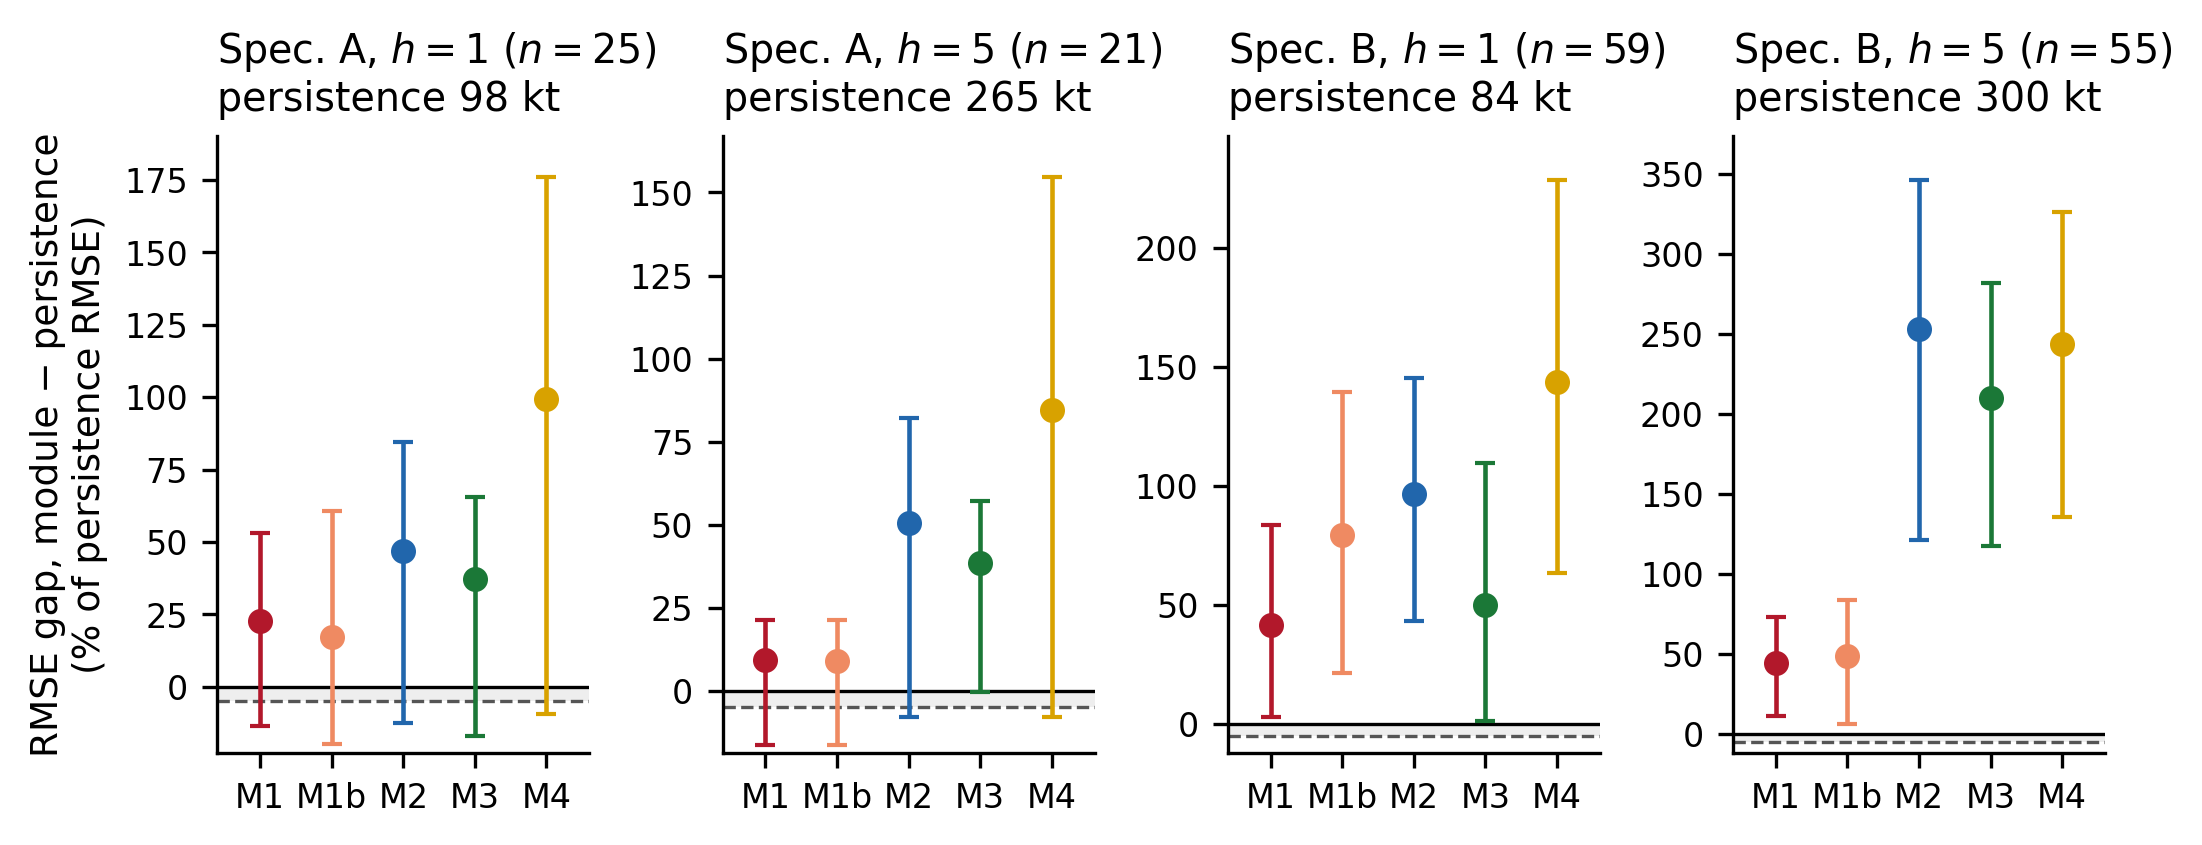
\includegraphics[width=\textwidth]{fig2_gaps}
\caption{Cod: persistence margins, RMSE of each module minus RMSE of origin-matched persistence as a percentage of the persistence RMSE, with 95\% paired moving-block bootstrap intervals (block $\max(h,3)$, 20\,000 replicates). The dashed line is the 5\% tie band; retention under (C2) requires the point estimate to lie below it. On Specification A every interval contains zero; on Specification B every interval lies above zero at the block length of the archived layer.}
\label{fig:gaps}
\end{figure}

The two specifications differ in what can be said about the margins. On Specification A every persistence margin has a bootstrap interval containing zero (M1 at one year: $+22.5\kt$, $[-13.4, +52.2]$, $p=0.19$; M3: $+36.6$, $[-16.8, +64.2]$, $p=0.93$), so the data do not show that the modules are worse than persistence, only that they are not demonstrably better; the five-year M3 margin is the nearest to significance ($+101.6$, $[-0.8, +151.4]$, $p=0.08$). On Specification B every persistence margin excludes zero at the archived block length (M1 at one year: $+35.0$, $[+2.7, +70.8]$, $p=0.03$; M3: $+42.3$, $[+1.0, +92.5]$, $p=0.04$; all five-year margins $p\le 0.02$). The M3 one-step margin on B is the only interval whose classification depends on the block length (SI S3). Re-running the catch-supplied modules with the consistent catch-timing convention, a sensitivity outside the archived protocol (SI S14), lowers their one-step RMSE by 20--75\,kt and their five-year RMSE by up to 16\%; M3 then stands 7\% above persistence at one year on A and 12\% on B, still outside the band, and every five-year margin remains far outside it. The verdict does not depend on the convention; the size of the one-step deficit does. The MAE columns show that the one-step deficit is concentrated in a few large errors: on Specification A the M3 MAE is 10\% above persistence where its RMSE is 37\% above. Where those errors sit is the next question.

\FloatBarrier
\subsection{Where the deficit arises}\label{sec:periods}

Protocol C is applied to the pooled score, but pooling averages over regimes that the stock did not average over. Table~\ref{tab:periods} splits the one-step rolling errors into the periods visible in Fig.~\ref{fig:series} and Fig.~\ref{fig:period} shows the per-origin errors behind it; the decomposition is post hoc and is reported as a description of the data, not as a second test. Three features emerge.

\begin{table}[!htb]
\centering\small
\caption{Cod: one-step rolling-origin RMSE (kt) by period of the forecast origin, with origin-matched persistence. Superscripts give the number of origins at which the module's forecast sits at the numerical floor ($<0.01\kt$), i.e.\ forecasts extinction; its absolute error is then the observed SSB. Bracketed values are paired bootstrap intervals for the module$-$persistence gap in kt (block 3, 20\,000 replicates; not shown for bands with $n<11$). Five-year values and the annual-landings pass are in SI S4.}
\label{tab:periods}
\resizebox{\textwidth}{!}{%
\begin{tabular}{@{}llrrrrrrr@{}}
\toprule
Spec. & Origins & $n$ & persist & M1 & M1b & M2 & M3 & M4 \\
\midrule
A & 1990--1995 (collapse) & 6 & 193.6 & 208.8$^{3}$ & 186.4$^{4}$ & 292.0 & 273.2$^{3}$ & 397.3 \\
A & 1996--2012 (low biomass) & 17 & 19.6 & 64.8$^{12}$ & 69.7$^{13}$ & 17.2 & 14.7 & 19.4 \\
A & 2013--2014 (early rebuild) & 2 & 66.7 & 122.7 & 138.9 & 32.4 & 28.6 & 38.1 \\
A & 1996--2014 pooled & 19 & 28.5 & 73.1 & 79.8 & 19.4 & 16.7 & 22.1 \\
 & \quad gap vs.\ persistence & & & $+44.6$ & $+51.3$ & $-9.1$ & $-11.8$ & $-6.4$ \\
 & \quad 95\% interval & & & $[+29, +60]$ & $[+29, +69]$ & $[-17, +7]$ & $[-20, +3]$ & $[-14, +9]$ \\
\midrule
B & 1965--1990 (fished, pre-collapse) & 26 & 94.7 & 142.4$^{2}$ & 186.4$^{3}$ & 184.2 & 166.3 & 260.6 \\
B & 1991--1995 (collapse) & 5 & 167.0 & 126.8$^{3}$ & 66.6$^{3}$ & 299.8 & 154.8$^{3}$ & 321.6$^{1}$ \\
B & 1996--2012 (low biomass) & 17 & 20.7 & 75.0$^{17}$ & 75.0$^{17}$ & 26.3 & 19.7 & 24.0 \\
B & 2013--2023 (rebuild) & 11 & 61.0 & 112.3 & 174.5$^{1}$ & 160.5 & 96.4 & 136.3 \\
B & 1996--2023 pooled & 28 & 41.5 & 91.5 & 124.0 & 102.7 & 62.3 & 87.4 \\
 & \quad gap vs.\ persistence & & & $+50.0$ & $+82.5$ & $+61.2$ & $+20.9$ & $+46.0$ \\
 & \quad 95\% interval & & & $[+26, +79]$ & $[+53, +118]$ & $[-2, +93]$ & $[-11, +47]$ & $[-5, +73]$ \\
\bottomrule
\end{tabular}}
\end{table}

\begin{figure}[!htb]
\centering
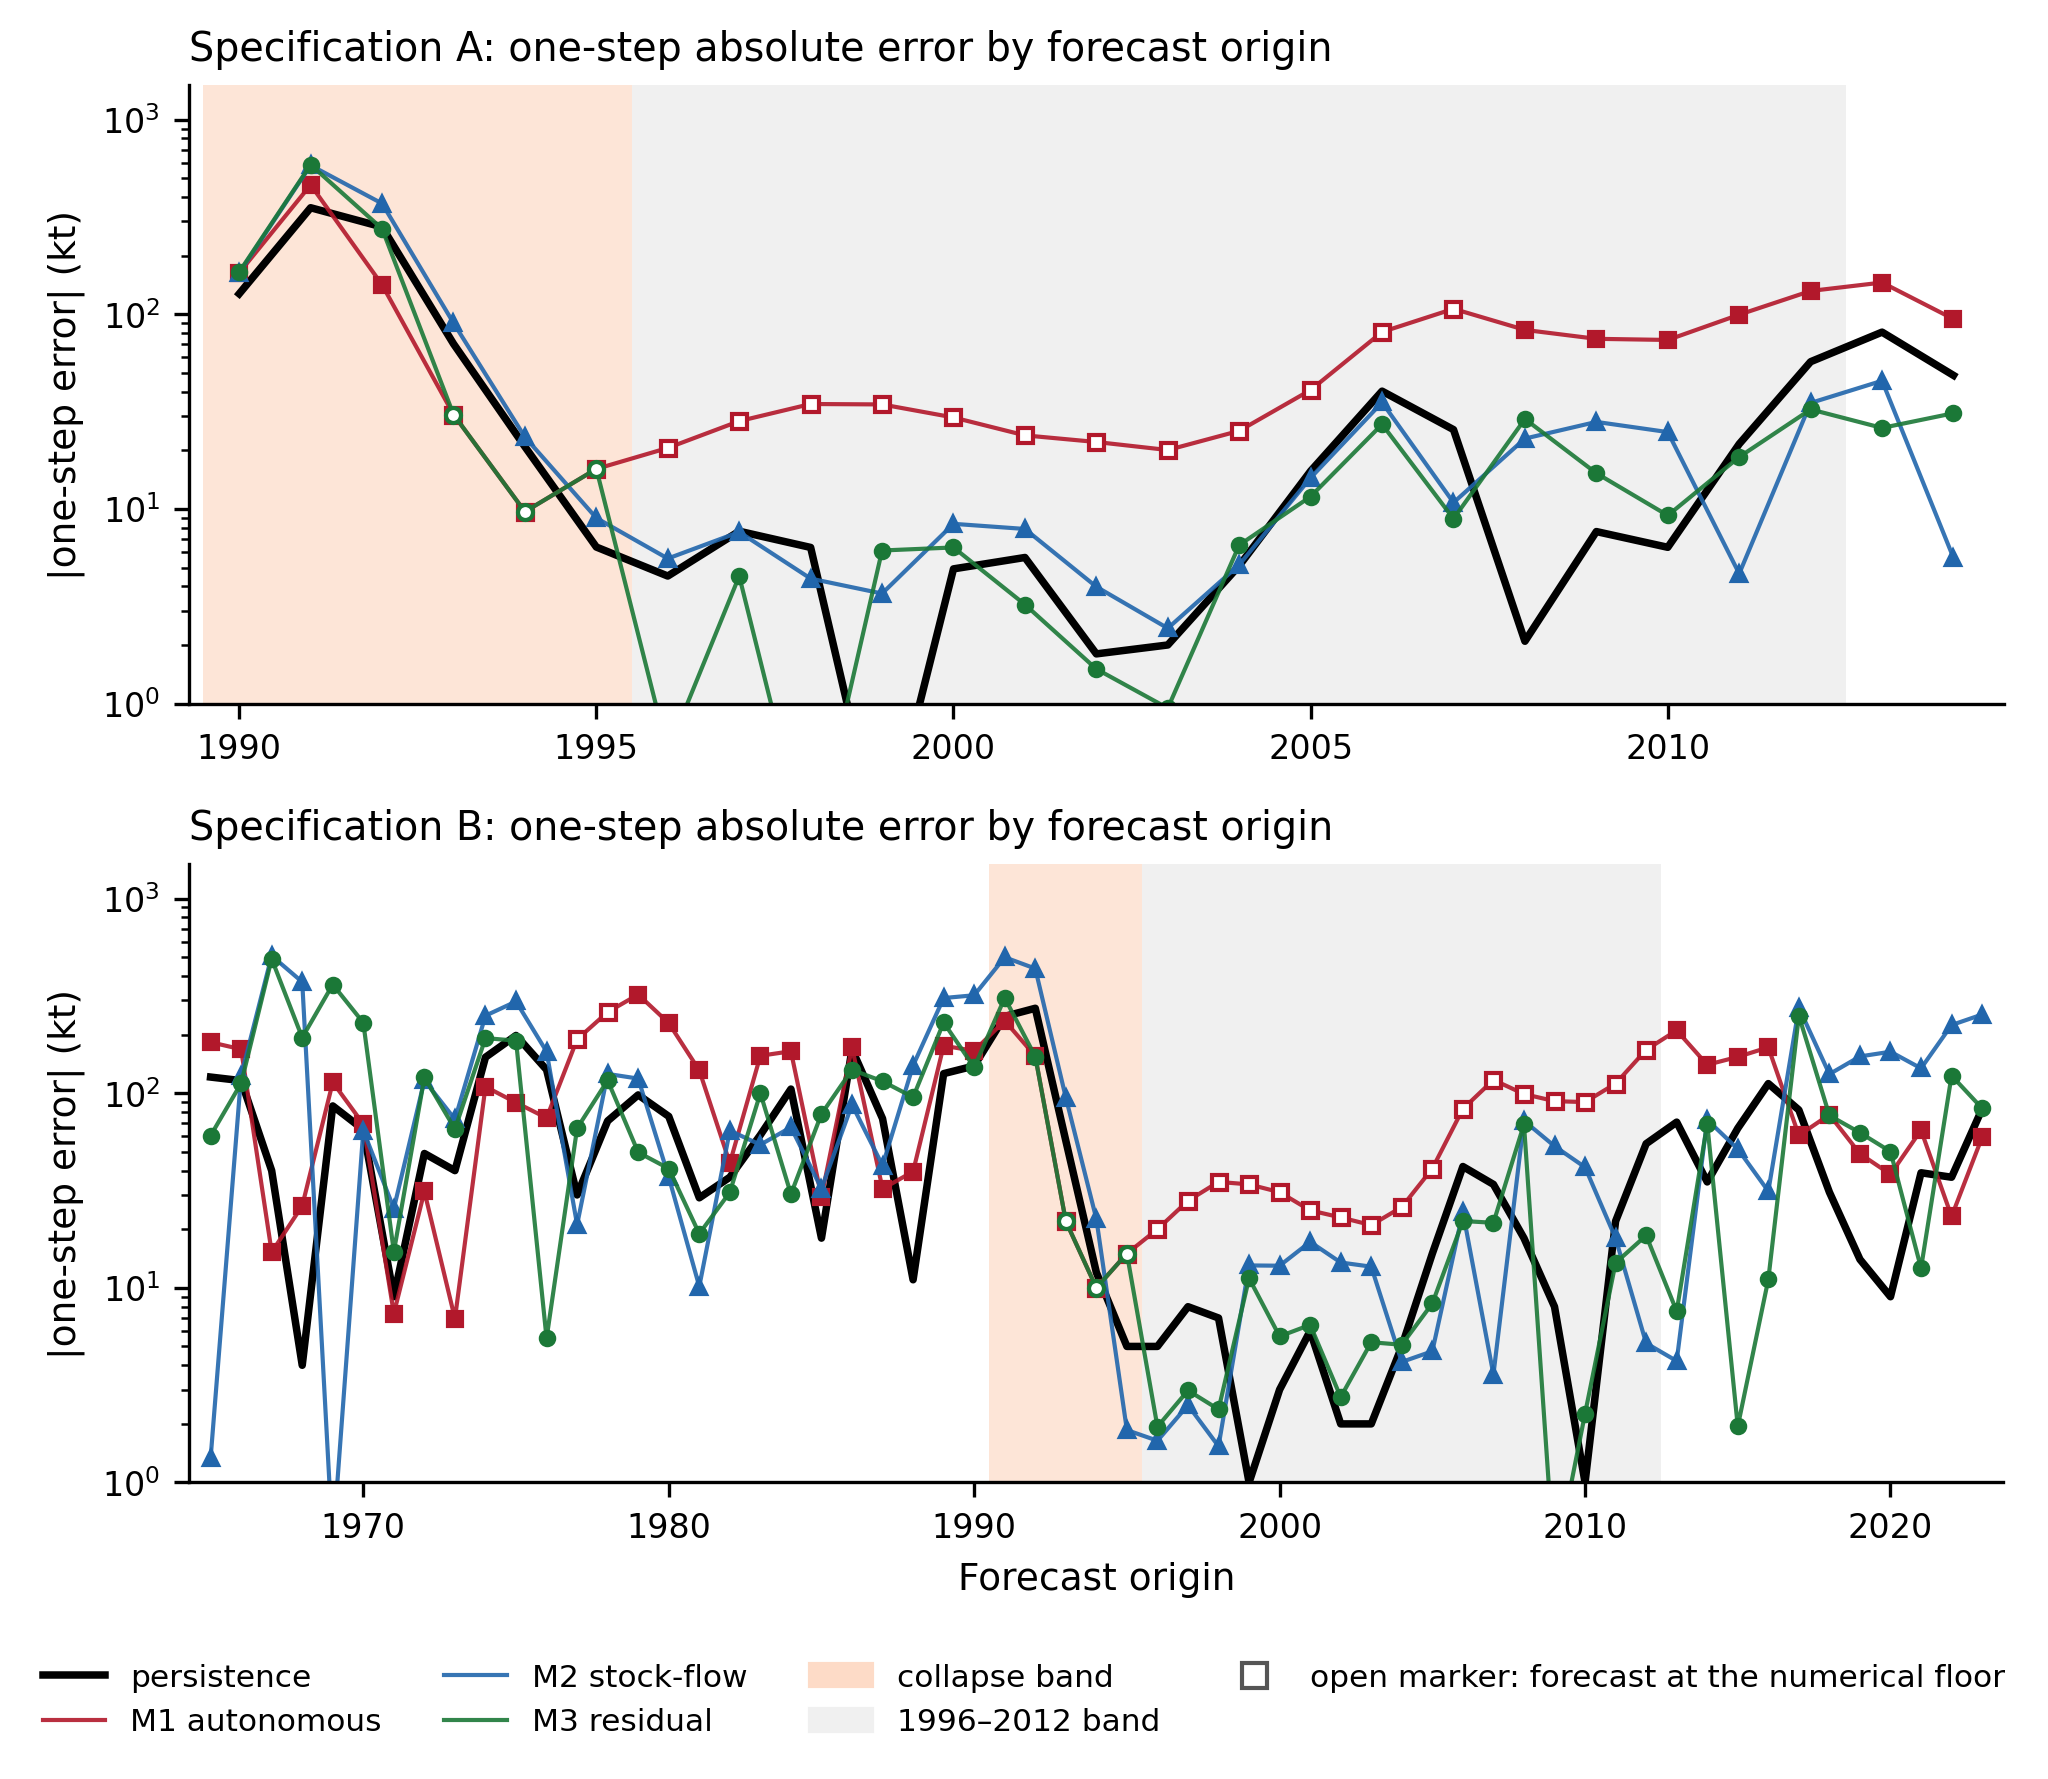
\includegraphics[width=\textwidth]{fig4_period}
\caption{Cod: one-step absolute error by forecast origin (log scale, floored at 1\,kt for display) for persistence, M1, M2 and M3 on (top) Specification A and (bottom) Specification B. Shading marks the collapse band and the 1996--2012 low-biomass band. Open markers are forecasts at the numerical floor: at those origins M1's error is simply the observed SSB, which is why its curve traces the stock trajectory through 1996--2012 on both panels.}
\label{fig:period}
\end{figure}

First, the pooled deficit is carried by the collapse band. On Specification A the six origins 1990--1995 contribute 94\% of the pooled one-step sum of squared persistence errors and 63--99\% of each module's; every forecaster is wrong by 130--590\,kt at the 1991 origin and by 140--710\,kt at the 1992 origin, because every forecaster, including persistence, extrapolates a state that is about to be removed. On Specification B the 26 fished pre-collapse origins add a second source of deficit: between 1965 and 1990 the catch-supplied modules are worse than persistence by 70--170\,kt, as a stock-flow model fitted to a series with 200--800\,kt removals mis-times the large swings of the 1960s and 1970s.

Second, the apparent collapse-band wins of M1, M1b and M3 on Specification B, and of M1b on A, are not forecasts of the collapse. At the 1993--1995 origins these modules forecast the floor: their training-mean catch (317--333\,kt on B, 177--208\,kt on A) exceeds the production of a stock of 10--100\,kt by an order of magnitude, so the map drives the state to $10^{-3}\kt$ in one step and the absolute error equals the observed value, which is small only because the stock was nearly gone. A floor forecast is a correct sign with no magnitude; it is credited by RMSE and should not be read as skill.

Third, the autonomous modules forecast extinction at every post-collapse origin, and the catch-supplied modules have one-step skill in the low-biomass regime on one specification only. Between 1996 and 2012 M1 and M1b sit at the floor at 17 of 17 origins on Specification B and at 12--13 of 17 on A; their RMSE in that band, 65--75\,kt against 20\,kt for persistence, is the root mean square of the observed SSB. Training-mean catch is a plug, not an estimate, and after a collapse it is a plug an order of magnitude above sustainable removals. In the same band M2, M3 and M4 forecast within 15--26\,kt, and on Specification A they beat persistence: pooling 1996--2014, M3 has one-step RMSE 16.7 against 28.5\,kt, a gap of $-11.8\kt$ ($-41\%$) with interval $[-20.5,+3.3]$, $p=0.19$. The intervals contain zero and the bands were chosen after the fact, but the point estimates are the right sign and the right order to be the residual signal that a catch-supplied production model should carry when the catch is small and the stock is far below $K$. On Specification B the same bands give the opposite answer: post-1995 every module is worse than persistence at one year and at five years by factors of 2--6, because the 2013--2023 rebuild, which Specification A does not contain, is forecast by the stock-flow modules as a rise several hundred kilotonnes above what occurred. The low-biomass skill does not transfer across the two series.

\FloatBarrier
\subsection{Why the collapse cannot be forecast from inside the class}\label{sec:identification}

The fixed windows (SI S4) show the behaviour the pooled scores summarise: from the 1983--1990 training window, in which SSB varied between 835 and 942\,kt, every module forecasts continuation, the autonomous modules holding the stock at the fitted equilibrium of 888.6\,kt and the catch-supplied modules, told that removals fall from 240 to 120 to 5\,kt, forecasting growth to about 1050\,kt by 1993 while the observed path falls from 862 to 9.7\,kt. This has a structural explanation that does not depend on the fitted values. Write $F_C(S) = \Spos{S + g(S) - C}$ for the deterministic map at catch $C$.

\begin{proposition}\label{prop:repeller}
Let $g$ be continuous with $g(0)=0$, let $C>0$, and let $S_-(C) = \inf\{S>0 : g(S)\ge C\}$, with $S_-(C)=\infty$ if the set is empty.
\begin{enumerate}[label=(\roman*),leftmargin=2.2em,itemsep=1pt]
\item Every trajectory of $F_C$ started in $[0,S_-(C))$ is nonincreasing and remains in $[0,S_-(C))$; on any interval on which $g \ge C$, $F_C(S)\ge S$, so a trajectory cannot decline in one step from a state in that interval.
\item A one-step decline larger than the removals, $S_{t+1} < S_t - C_t$, requires $g(S_t) < 0$. On the compensatory branch this is impossible for $0\le S_t\le K$, whatever $(r,K)$; on the depensatory branch it requires $S_t < \sA$.
\end{enumerate}
\end{proposition}

The proof is in \ref{app:proofs}. For the Schaefer branch with $4C\le rK$, $S_-(C) = \tfrac{K}{2}\bigl(1-\sqrt{1-4C/(rK)}\bigr)$ is the lower, unstable equilibrium and $S_+(C)=K-S_-(C)$ the upper, stable one, with $g\ge C$ between them; for $4C>rK$ production never reaches the catch and every trajectory declines to the floor. Three consequences follow. First, the lower equilibrium is generated by the catch: it vanishes as $C\to 0$ and it exists on the compensatory branch with no depensation term at all, so a threshold below which the autonomous map declines is a statement about sustained removals, not about the biology of small populations. Second, the 1990 state, 862\,kt, lies between $S_-=144$ and $S_+=888.6\kt$ for the fitted map under 240\,kt, so by (i) the autonomous forecast cannot decline at all; it rises to the attractor, which is locally stable ($F_C'(S_+)=-0.39$). Third, and independently of any fit, the 1991, 1992 and 1993 transitions are declines larger than the recorded catch: apparent net production $S_{t+1}-S_t+C_t$ is $-113$, $-161$ and $-66\kt$ under the coarse regime and $-181$, $-240$ and $-59\kt$ under annual landings (Fig.~\ref{fig:production}). By (ii) no parameter value of the compensatory branch, and no catch-supplied module built on it, can reproduce these steps; the depensatory branch can do so only with a threshold $\sA$ above 735\,kt, which no fit approaches. The collapse lies outside the model class at the recorded catch. The assessment model itself accommodates these years through under-reported catch and an elevated natural mortality \citep{Cadigan2016}; a forecaster that takes the catch record as given cannot, and a forecaster that is told the catch is falling to 5\,kt forecasts growth.

\begin{figure}[!htb]
\centering
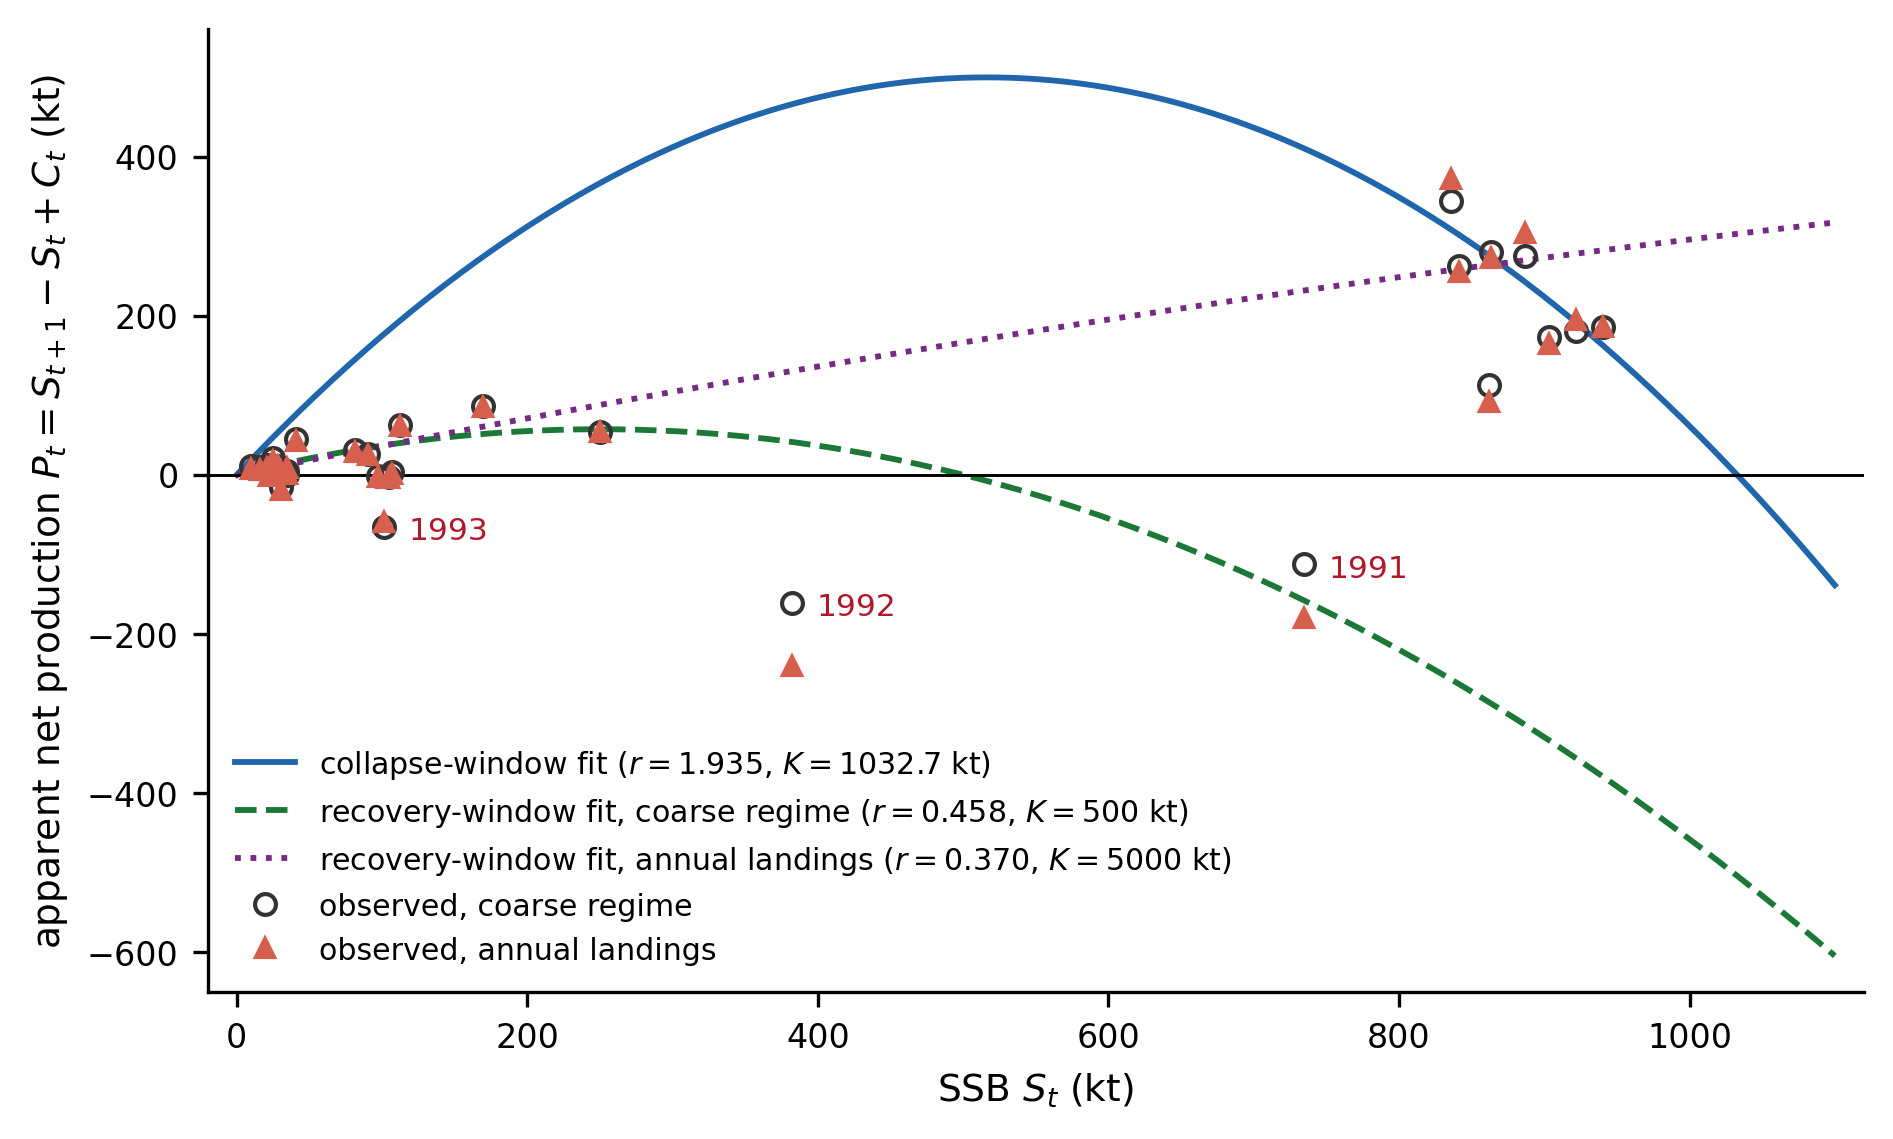
\includegraphics[width=0.9\textwidth]{fig5_production}
\caption{Cod: apparent net production $S_{t+1}-S_t+C_t$ against $S_t$ on Specification A, with the collapse-window fit ($r=1.935$, $K=1032.7$; maximum $rK/4=500\kt$ at $S=516$) and the two recovery-window fits. Under 240\,kt of removals the collapse-window map has its repeller at $S_-=144\kt$ and its attractor at $S_+=889\kt$. The 1991--1993 transitions lie below every nonnegative production curve: the stock lost more biomass than the recorded catch removed. The recovery-window fits are nearly linear through the low-biomass points, with $K$ at its initialiser (500\,kt, coarse regime) or at its upper bound (5000\,kt, annual landings).}
\label{fig:production}
\end{figure}

The depensatory branch does not change this. In the fixed windows, which exclude the collapse transitions from training, M1b's $\sA$ estimate sits at its lower bound of zero, and the profile of the objective over $\sA$ changes by 3--7\% across its whole range (SI S5). In rolling fits whose training window contains the collapse, the estimate jumps to 585--734\,kt on Specification A at every origin from 1992 to 2010 and falls back to 5\,kt from 2011, while on Specification B it stays at zero throughout (SI S5). A depensation parameter that is zero, 700\,kt or 5\,kt depending on the window is not an estimate of an Allee threshold; it is the branch's only means of absorbing transitions the class cannot otherwise represent. Whether depensation has delayed the recovery \citep{Shelton1999,Hutchings1996,Rose2026} is therefore not a question this test can answer, and the usual difficulty of detecting depensation from assessment series \citep{Myers1995,Liermann1997} is compounded by a collapse that the class attributes to it by default. The compensatory fits are weakly identified as well: $K$ rests at its 5000-kt bound at 23 of the 25 Specification A origins from 1992 onward, so the post-collapse stock-flow forecaster is in effect linear, $S_{t+1}\approx(1+r)S_t-C$ with $r\approx0.25$ (A) and $0.50$ (B), the familiar outcome of fitting a production model to a series with little contrast \citep{HilbornWalters1992,LudwigWalters1985,Polacheck1993}. That linear growth term is the whole of the low-biomass skill reported in Section~\ref{sec:periods}.

\FloatBarrier
\subsection{Operating characteristics of Protocol C}\label{sec:operating}

Fig.~\ref{fig:operating} reports the retention frequencies under the seven data-generating processes of Section~\ref{sec:power}. When the truth is the autonomous Schaefer module at collapse-window parameters (D1), the rule retains M1 in 96.5\% and 98.5\% of replicates at the two noise levels: the empirical non-retention of M1 is not a power failure. At recovery-window parameters (D2) power is 71\% at the lower noise and 13\% at the higher; for the stock-flow truth (D3) it is 9--11\% and for the depensatory truth (D4) 0.5--1.5\%. Under the persistence-true null (D5) false retention is 1.5--3.0\%, within the bar. The two processes outside the class fail the specificity bar badly: a drifting-productivity truth (D6) leads to retention of some module in 68--76\% of replicates and a smooth path observed with error (D7) in 93--98\%, most often M1. The rule is therefore specific against the absence of structure but not against the presence of structure of another kind; it detects that something beyond persistence is present, not that the retained module is that something. Alternative decision rules evaluated on the same replicates (SI S8) show that the 5\% band carries most of the specificity (removing it costs 0.21 of specificity for 0.06 of power), that the comparator hurdle costs 0.10 of power for 0.006 of specificity, that a MASE-type criterion alone \citep{HyndmanKoehler2006} is more powerful and far less specific, and that an information criterion penalising parameter count dominates the adopted rule on both axes within the class.

\begin{figure}[!htb]
\centering
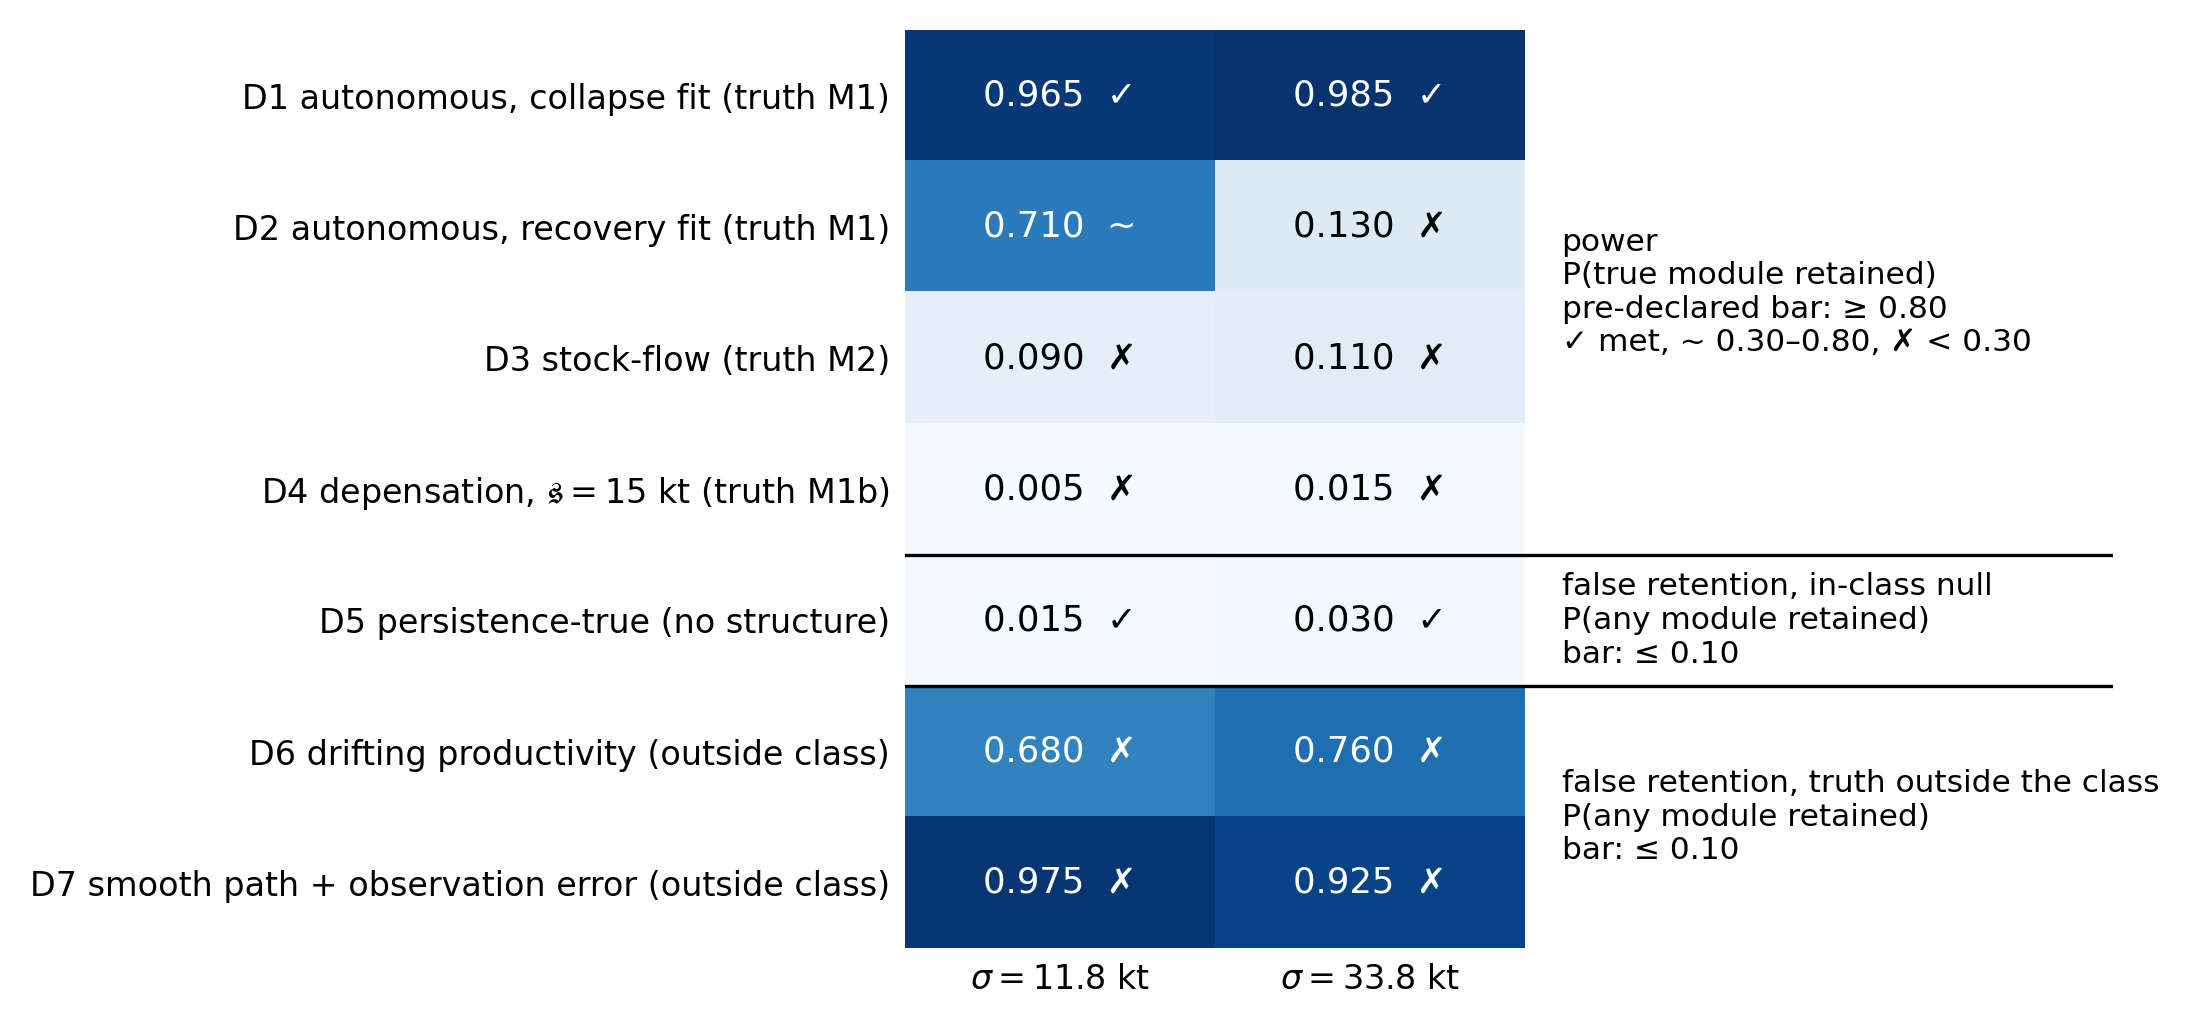
\includegraphics[width=\textwidth]{fig6_operating}
\caption{Cod: retention frequencies of Protocol C under seven data-generating processes (200 replicates each, two process-noise levels; Specification A design). D1--D4: fraction of replicates in which the truth-matching module is retained (power; pre-declared bar 0.80). D5: fraction in which any module is retained under a persistence-true null (false retention; bar 0.10). D6--D7: the same under truths outside the ladder's class.}
\label{fig:operating}
\end{figure}

\FloatBarrier
\subsection{Variant passes and the years after 2015}\label{sec:verdict}

Four variant passes were added after the primary pass and declared in order (SI S1, S4), each scored against persistence recomputed on its own origin set: annual landings in place of the coarse regime (M2 160.4, M3 153.6, M4 206.3\,kt at one year against 98.0 for persistence); a survey-scaled start value (128.1 and 331.0\,kt); a two-regime intrinsic rate with a 1991 break at the capelin collapse \citep{Buren2014,DFO2024b} (153.8 and 334.0\,kt on A; 146.8 and 894.4 on B); and a capelin acoustic-index multiplier on the years with an acoustic estimate \citep{Murphy2025,NAFC2025} (150.0 and 262.3\,kt on A against 96.6 and 193.0 for persistence on the reduced set). No variant comes within the band at either horizon.

Specification A ends in 2015, and the continuation of the same assessment family is published in the RAM Legacy database \citep[v4.66, stock COD2J3KL;][]{Ricard2012}, with xteNCAM reading the same years independently (SI S11). The outcome window is an increase regime: every year 2016--2021 lies above its 2015 origin in both vintages, so it contains no event of the kind the collapse test probes, and persistence from the 2015 origin errs low throughout (RMSE 133.3\,kt on the RAM vintage). The two vintages agree on the outcome years to within 1--26\,kt while on the historical overlap they do not (the Table A2 vintage runs 24.7\,kt above the RAM vintage on average over 1983--2015, with a maximum difference of 131\,kt), so that the LRP defined as the 1983--1989 mean is 884.6\,kt on one vintage and 790.0\,kt on the other; the two thresholds classify the same xteNCAM file differently in 29 of 71 years; and the 2023 framework revision moved the reported zone from critical to cautious without a change in the stock \citep{DFO2024a,Regular2025}. Over the same period the observing system lapsed: partial fall-survey coverage in 2021 and 2022 left the leading indicator uncomputable, no typical assessment update was possible in 2022 or 2023, and the survey vessel was condemned (SI S12). None of this touches the RMSE comparison, which never uses a threshold; all of it bears on the verdict any forecast is scored against, and after 2015 the reference-point and observation layers moved more than forecast skill did.

\subsection{Reading the cod verdict}\label{sec:codreading}

A negative verdict from a scored test carries the weight of the test's power, and Section~\ref{sec:operating} lets that weight be assigned per module. For M1 the verdict is strong: at the parameters of the series on which it was tested the rule retains a true autonomous Schaefer module in 97--99\% of replicates, so its non-retention on both specifications, with a persistence margin that excludes zero on Specification B, is evidence that an autonomous production model driven by mean historical catch does not describe this stock's year-to-year SSB transitions. For M2, M3 and M4 the verdict is weak: against a true stock-flow process at recovery-window parameters the rule has 9--11\% power, so non-retention is compatible with a catch-supplied structure being present and too faint to clear a 5\% band at both horizons; the low-biomass skill on Specification A is consistent with that reading, and its failure to extrapolate is evidence that what the modules carry is a short-memory growth term. For M1b the verdict is not about depensation at all: the parameter it adds is unidentified, and the test could not have retained a true depensatory module. Three features of assessment output make persistence a demanding benchmark on an assessed state, and they are the reason this paper scores on the state: the series is a retrospective estimate smoothed by the assessment's process-error structure, so the last value is an efficient summary of the recent past; the forecaster is fitted to the same smoothed series and learns slow dynamics, then adds a parametric shape and a catch plug the series does not demand; and the quantity that moves the series most, the collapse, is one that no member of the class can reproduce at the recorded catch, so the model carries the full persistence error there and adds its own. Hindcast cross-validation on the fitted index \citep{Kell2016,Kell2021,Carvalho2021} answers whether the assessment predicts its own data, which is a different and easier question than whether its dynamics predict next year's biomass.
\FloatBarrier
\section{System II: Edwards Aquifer, index well J-17}\label{sec:edwards}

\subsection{Data and specification}\label{sec:edw_data}

The predictand is the calendar-year mean of daily-high elevation at well J-17 (TWDB 6837203, EAA AY-68-37-203), the index well of the San Antonio Pool of the Edwards (Balcones Fault Zone) Aquifer, for 1934--2023 (Table~\ref{tab:edwspec}, Fig.~\ref{fig:edwseries}). Three hydrological objects are read off this one number and should be kept apart: the head is observed at an access point; it indexes a store of water, which is the resource; and the store is replenished and drawn by fluxes, which are the flow. The one-pool water balance closes this loop approximately, in the increment-structure sense used throughout: head change equals weighted fluxes plus a linear drain. It is not a closed mass balance. Annual means use all available daily highs; no year falls below the 240-observation floor (minimum $n=242$ in 1939); missing days are not interpolated; the published pre-continuous composite is used as issued; and the 2023 values carry provisional status. Recharge $R$ is USGS total San Antonio-area recharge ($10^3$ acre-ft\,yr$^{-1}$), estimated by the stream-loss method of \citet{Puente1978} and constructed independently of J-17 \citep{UmphresChoi2025}; pumpage $P$ is well discharge from Edwards Aquifer Authority Table 1 \citep{EAA2024}. Both are constructed fluxes, not observations of J-17, and total-area values mix the San Antonio and Uvalde pools. Spring discharge is stored and not used as a driver. Climate predictors, used only by the climate-informed variants, are September--November Ni\~no~3.4 (HadISST) and calendar-year precipitation in Texas climate divisions 06 and 07 (NCEI nClimDiv). Two thresholds frame the series without entering any forecast: the Edwards Aquifer Authority's Stage~I line (10-day mean J-17 below 660\,ft, a 2007 institutional rule) and the physical level near 618\,ft at which Comal Springs approaches cessation (1956 daily minimum 612.51\,ft). The annual mean is below 660\,ft in 31 of 90 years; the daily minimum is below 618\,ft in one (1956).

\begin{table}[!htb]
\centering\small
\caption{The J-17 specification. D = data, E = empirical construct, M = model, N = normative threshold. The predictand is a measured well series, not a storage reconstruction, a numerical-model inversion, the J-27 Uvalde index or spring discharge.}
\label{tab:edwspec}
\begin{tabularx}{\textwidth}{@{}>{\raggedright\arraybackslash}p{0.24\textwidth}Lc@{}}
\toprule
Field & Contents & Type \\
\midrule
System & Edwards Aquifer, San Antonio Pool, indexed by J-17 & D \\
Predictand $H_t$ & calendar-year mean of daily-high J-17 elevation (ft AMSL), 1934--2023 (90 years) & D \\
Drivers & recharge $R_t$ (USGS, stream-loss method); pumpage $P_t$ (EAA Table 1) & D/E \\
Physical threshold & head at which Comal Springs does not cease ($\approx$618\,ft) & N/E \\
Institutional threshold & EAA Stage I, 10-day mean $<660$\,ft (in force after 2007); the annual-mean indicator is a coarse proxy & N \\
Disturbance & recharge pulses; unmodelled karst; Uvalde--San Antonio exchange & M \\
Service series & USGS 08168710 Comal Springs annual-mean discharge (cfs); scored after retention is frozen & D \\
Fixed windows & drought-of-record drawdown (train 1934--1950, test 1951--1956); drought-of-record recovery (1934--1956 / 1957--1961); pre-permit wet interval (1980--1990 / 1991--1995); critical-period era (1997--2014 / 2015--2023) & --- \\
Rolling origins & minimum 15 training years; $n=75$ ($h=1$), $n=71$ ($h=5$); every model on identical origin sets & --- \\
\bottomrule
\end{tabularx}
\end{table}

\begin{figure}[!htb]
\centering
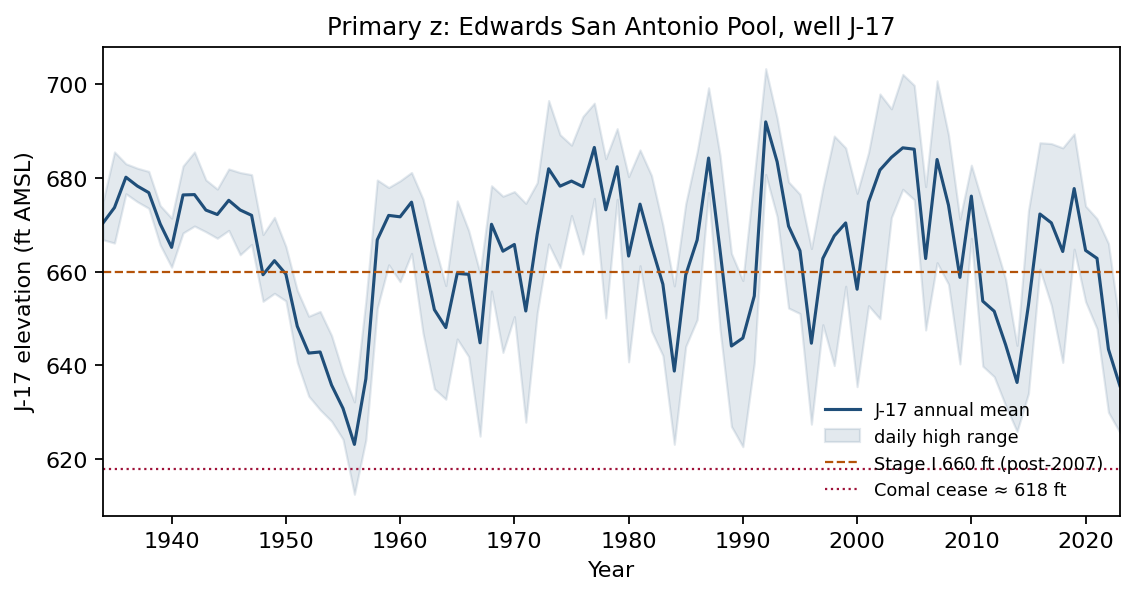
\includegraphics[width=0.92\textwidth]{edw_fig1_series}
\caption{J-17 annual mean and daily-high range, 1934--2023. 1956 mean 623.15\,ft (daily minimum 612.51\,ft); 1992 mean 691.96\,ft (daily maximum 703.31\,ft); 2023 mean 635.68\,ft. The annual mean is below the 660-ft Stage I line in 31 of 90 years.}
\label{fig:edwseries}
\end{figure}

\subsection{The water-balance ladder}\label{sec:edw_ladder}

\begin{definition}[One-pool water-balance map]\label{def:pool}
With head clipped to $[610,710]$\,ft, the one-pool map is
\begin{equation}\label{eq:pool}
H_{t+1} \;=\; \bigl[\,H_t + \alpha + \beta\tilde R_{t+1} + \gamma\tilde P_{t+1} + \delta H_t\,\bigr]_{\mathrm{clip}},
\end{equation}
where $\tilde R$ and $\tilde P$ are the flux values a forecast substitutes for the unknown year-$(t+1)$ fluxes. Forecasts are issued at the end of year $t$ from $(H,R,P)$ through $t$; $(\alpha,\beta,\gamma,\delta)$ are refitted by least squares on the training transitions at every origin.
\end{definition}

The clip stands in for a physical storage floor; it never binds on the observed record (annual means 623--692\,ft) and binds only on persisted-drought forecast paths, where it does real work (SI S17). The ladder (Table~\ref{tab:edwladder}) differs from the cod ladder in one structural respect that Section~\ref{sec:synthesis} turns on: the causal rungs must \emph{substitute} something for the target-year fluxes. M2 persists last year's $(R_t,P_t)$; M2m substitutes the training-mean fluxes; M3 adds an AR(1) residual on $\Delta H$ to M2; M4 is a one-year information-delay variant kept as a symmetry control with the cod ladder (J-17 is a telemetered gauge, so the module prices a theoretical lag rather than a constraint of this system). The climate-informed variants replace persisted $R$ by a one-step forecast of $R$ from information known at $t$: an AR(1) on $R$, lagged Ni\~no~3.4, lagged climate-division precipitation, or all three; for $h>1$ the one-step recharge forecast is held constant. The oracle receives the realised $(R_{t+h},P_{t+h})$ and is excluded from retention, as is a precipitation oracle. M1 is the univariate AR(1), $H_{t+1}=a+\varphi H_t$, scored as the autonomous rung.

\begin{table}[!htb]
\centering\small
\caption{The J-17 ladder. ``Comparator'' is the next-simpler causal model under (E2); M1 has none and is tested against persistence only.}
\label{tab:edwladder}
\begin{tabularx}{\textwidth}{@{}>{\raggedright\arraybackslash}p{0.13\textwidth}>{\raggedright\arraybackslash}p{0.16\textwidth}>{\raggedright\arraybackslash}p{0.2\textwidth}L>{\raggedright\arraybackslash}p{0.14\textwidth}@{}}
\toprule
ID & Class & Fluxes substituted at $t+h$ & Role & Comparator \\
\midrule
persist & baseline & --- & $\hat H_{t+h}=H_t$ & --- \\
mean & baseline & --- & training-window mean & --- \\
M1 & autonomous AR(1) & --- & $H_{t+1}=a+\varphi H_t$ & (persistence only) \\
M2 & causal stock-flow & last $(R_t,P_t)$ persisted & candidate for retention & M1 \\
M2m & climatological stock-flow & training-mean $(\bar R,\bar P)$ & affine AR(1) by class & M1 \\
M3 & residual & as M2 & AR(1) residual on $\Delta H$ & M2 \\
M4 & delay & as M2 & information lag; symmetry control & M3 \\
M2\_Rar, M2\_Renso, M2\_Rprecip, M2\_combo & climate-informed & one-step forecast of $R$ (AR(1) on $R$; Ni\~no~3.4; precipitation; all three) & climate rung & M1 (declared) \\
M2\_oracle & diagnostic & realised $(R,P)$ & nowcast ceiling; excluded & --- \\
\bottomrule
\end{tabularx}
\end{table}

\begin{remark}[Class reduction of M2m]\label{rem:class}
Under constant fluxes $\tilde R_{t+1}=\bar R$, $\tilde P_{t+1}=\bar P$, the map \eqref{eq:pool} reduces to $H_{t+1}=(1+\delta)H_t+\mathrm{const}$ and therefore shares M1's forecast function class, though not its estimator: M2m pins its intercept from the in-sample mean fluxes, an additional identifying use of the recharge and pumpage records, while the persistence coefficient $(1+\delta)$ is not mean-flux dependent. The decision to decline M2m on these grounds is a protocol choice recorded in the frozen documents, not a consequence of (E1)--(E2).
\end{remark}

\FloatBarrier
\subsection{The verdict under Protocol E, and under Protocol C}\label{sec:edw_verdict}

Table~\ref{tab:edwrolling} gives the rolling-origin summary and Fig.~\ref{fig:edwrmse} the per-model RMSE at both horizons. At $h=1$ persistence scores 13.23\,ft and the training mean 16.17\,ft. M1 scores 12.84\,ft and satisfies (E1); as the simplest autonomous model it has no next-simpler causal comparator, so (E2) is vacuous and M1 is retained by the point rule. M2 (14.70), M3 (14.46) and M4 (14.30\,ft) each fail (E1): the causal balance that persists last year's fluxes is worse than persisting the head. M2m (12.28\,ft) satisfies (E1) and, against M1, (E2); it is listed and then declined by the class clause. The oracle, at 7.55\,ft, is 43\% below persistence and is excluded. Under Protocol E, therefore, one output-only module is retained and no stock-flow, residual or delay module is. Under Protocol C, restated on the same scores, nothing is retained: M1's 2.96\% margin lies inside the 5\% band, and at $h=5$ M1 (21.25\,ft) does not beat persistence (21.11\,ft) at all. The two protocols disagree about M1 and agree about everything else, and both readings are reported because both are true of the scores.

\begin{table}[!htb]
\centering\small
\caption{J-17: rolling-origin summary (ft; $n=75$ at $h=1$, $n=71$ at $h=5$, identical origin sets for every row) and the retention decision under Protocol E. Subscripts give the horizon; $\Delta$ columns are $h=1$ RMSE differences, negative favouring the module. The training mean is the best non-oracle forecaster at $h=5$.}
\label{tab:edwrolling}
\footnotesize\setlength{\tabcolsep}{3.5pt}
\begin{tabularx}{\textwidth}{@{}>{\raggedright\arraybackslash}p{0.19\textwidth}rrrrrL@{}}
\toprule
Model & RMSE$_1$ & MAE$_1$ & RMSE$_5$ & $\Delta$ persist & $\Delta$ M1 & Protocol E decision \\
\midrule
persist & 13.23 & 10.73 & 21.11 & --- & --- & benchmark \\
mean & 16.17 & 13.17 & \textbf{16.80} & $+2.94$ & --- & benchmark \\
M1 AR(1) & 12.84 & 10.72 & 21.25 & $-0.39$ & --- & retained (point rule; margin within noise) \\
M2 persisted fluxes & 14.70 & 11.45 & 33.49 & $+1.47$ & $+1.86$ & rejected: fails (E1) \\
M2m climatological fluxes & 12.28 & 10.22 & 17.44 & $-0.95$ & $-0.56$ & passes (E1), (E2); declined by class clause \\
M3 residual & 14.46 & 11.12 & 33.46 & $+1.23$ & $+1.62$ & rejected \\
M4 delay & 14.30 & 11.17 & 33.39 & $+1.07$ & $+1.46$ & rejected \\
M2\_oracle & 7.55 & 5.79 & 10.86 & $-5.68$ & --- & excluded (uses future $R,P$) \\
\bottomrule
\end{tabularx}
\end{table}

\begin{figure}[!htb]
\centering
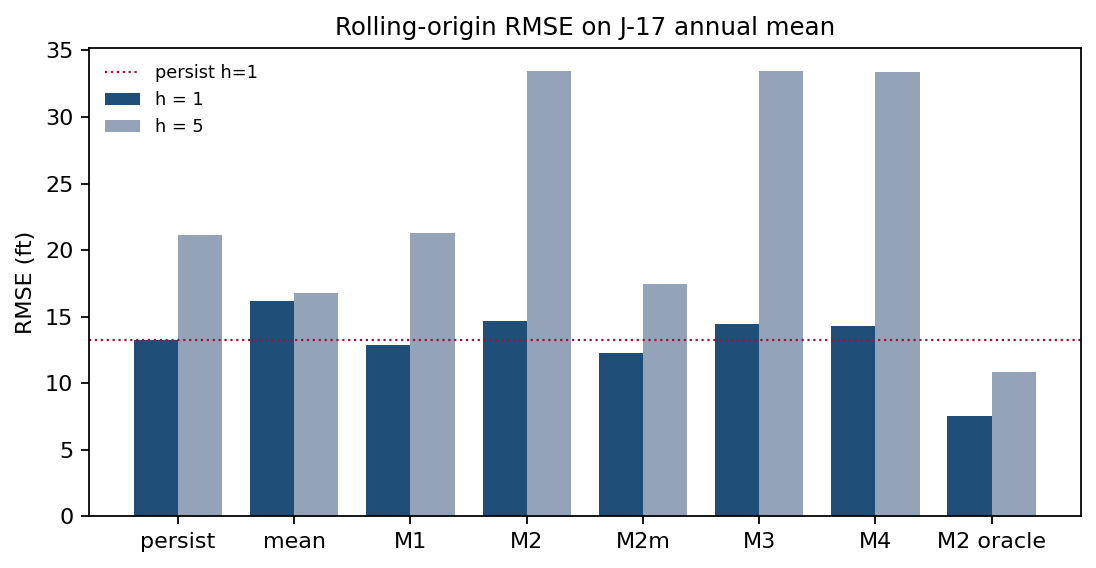
\includegraphics[width=0.8\textwidth]{edw_fig3_rmse}
\caption{J-17: rolling-origin RMSE by model at $h=1$ and $h=5$. The oracle is a diagnostic ceiling and is excluded from retention. At five years the training mean is the best non-oracle forecaster and M2--M4 are 60\% worse than persistence.}
\label{fig:edwrmse}
\end{figure}

The retention of M1 is a one-year, point-RMSE statement and should be read as such. The margin is 0.39\,ft on $n=75$; MAE is a tie (10.72 against 10.73\,ft); at five years the ordering reverses; and at the decision scale of annual drought-stage declarations the difference is operationally nil. The record of the class clause is as important as the retention: on the rule as written, the statement ``no stock-flow module is retained'' is an artefact of declining M2m, since the water-balance-identified affine map with climatological fluxes is the best one-step forecaster tested. What the ladder actually shows is that \emph{persisting last year's recharge} is the failure, not the balance as such; Section~\ref{sec:edw_mech} and Proposition~\ref{prop:increment} make that statement exact.

\subsection{Uncertainty on the margins}\label{sec:edw_uncertainty}

Table~\ref{tab:edwdm} attaches Diebold--Mariano statistics and moving-block bootstrap intervals to the load-bearing margins, computed from the archived per-origin forecast files; the layer is post-freeze and changes no verdict. Three readings follow. The retention margin itself (M1 $-$ persist, $-0.39$\,ft) is within noise, as are the M2m-over-M1 estimator margin and the M2 causal loss (the last borderline, its interval touching zero); the only one-year margin that separates from zero is M2m over persistence ($-0.95$\,ft, $p=0.003$). The five-year climatology win ($-4.30$\,ft) is robust: its bootstrap interval excludes zero, and the $h=5$ Diebold--Mariano $p$ of 0.10 reflects the known under-sizing of that statistic under overlapping origins. And the climate-rung margins are within noise in both directions. An independent second implementation of the layer (different seed, block length $h$, 20\,000 replicates, different HAC weighting and variance convention; SI S18) reproduces every reading: M1's retention margin has $z=-0.86$ and block interval $[-1.22,+0.56]$\,ft; the M2m edge over persistence has $p=0.001$; the five-year climatology win has $p=0.035$.

\begin{table}[!htb]
\centering\small
\caption{J-17: uncertainty on the load-bearing margins (post-freeze layer; Diebold--Mariano with Newey--West HAC at lag $h-1$; paired moving-block bootstrap, block length 8, 10\,000 replicates, seeded). Rolling origin, $h=1$ unless noted.}
\label{tab:edwdm}
\scriptsize\setlength{\tabcolsep}{3pt}
\begin{tabular}{@{}lrrrcl@{}}
\toprule
Comparison & margin (ft) & DM & $p$ & 95\% block CI (ft) & separates \\
\midrule
M1 $-$ persist & $-0.39$ & $-0.85$ & 0.40 & $[-1.51,\,+0.71]$ & no \\
M2m $-$ persist & $-0.95$ & $-3.07$ & 0.003 & $[-1.45,\,-0.68]$ & \textbf{yes} \\
M2m $-$ M1 & $-0.56$ & $-1.61$ & 0.11 & $[-1.53,\,+0.13]$ & no \\
M2 $-$ persist & $+1.47$ & $+1.27$ & 0.21 & $[-0.02,\,+3.40]$ & no (borderline) \\
mean $-$ persist ($h=5$) & $-4.30$ & $-1.65$ & 0.10 & $[-9.72,\,-2.09]$ & \textbf{yes} \\
M1 $-$ persist ($h=5$) & $+0.15$ & $+0.06$ & 0.95 & $[-5.57,\,+4.94]$ & no \\
M2\_combo $-$ M1 (climate) & $-0.13$ & $-0.21$ & 0.83 & $[-1.37,\,+1.31]$ & no \\
M2\_combo $-$ M2m (nested) & $+0.43$ & $+0.74$ & 0.46 & $[-0.56,\,+1.57]$ & no \\
\bottomrule
\end{tabular}
\end{table}

\FloatBarrier
\subsection{The mechanism: a near-white driver, a nowcasting map, and what climate indices add}\label{sec:edw_mech}

The one-pool increment tracks same-year recharge: $r(\Delta H_t,R_t)=0.74$ on the 1934--2023 record, and the oracle's RMSE is 43\% below persistence at $h=1$ and 49\% below at $h=5$. The same increment is almost unrelated to last year's recharge ($r(\Delta H_t,R_{t-1})=0.06$), because annual recharge has almost no memory: $r(R_t,R_{t-1})=0.17$ against 0.87 for pumpage. A module that persists $R_t$ therefore persists a quantity that does not persist, and it loses to persisting the head itself; given the year's realised fluxes the same map is a nowcast of the year's head at 7.55\,ft. That is the diagnostic that separates a forecasting failure from a structural one: the balance accounts for the contemporaneous increment, and it has nothing to say about next year's increment because next year's recharge is not in any information set at the origin.

The fixed windows make the point visibly (SI S17). The 1957--1961 recovery from the drought of record is a recharge pulse ($R_{1956}=43.7$, $R_{1957}=1142.6\times10^3$ acre-ft): persistence stays at the 1956 floor (RMSE 43.6\,ft), M2 persists drought recharge and falls further, into the clip (55.3\,ft), and the oracle tracks the rise (12.3\,ft). The 1992 peak and the 2015--2023 window repeat the split. On the 1951--1956 drawdown M2 ``beats'' the oracle (18.1 against 19.7\,ft), but for a reason that undermines it: the map trained on 1934--1950 has the wrong sign on pumpage ($\gamma=+0.021$), because pumping rose as the drought deepened and least squares aliases the human response into the state transition.

The climate-informed variants ask whether the signals observable at the annual origin (September--November Ni\~no~3.4, lagged climate-division precipitation, an AR(1) on $R$) supply a recharge forecast that closes the gap (Table~\ref{tab:edwclimate}). They do not. On the recharge target itself the climate modules have modest skill relative to climatology (528--545 against $556\times10^3$ acre-ft; persisted recharge 702), and the autoregression on near-white recharge has none. On the head, the three climate modules beat persistence and M1 by 0.02--0.13\,ft, margins within noise (Table~\ref{tab:edwdm}); at $h=5$ all three are 3--6\,ft worse than persistence, a design consequence of holding the one-step recharge forecast constant over the horizon; and against the nested climatological-flux baseline M2m they lose outright (12.71--12.82 against 12.28\,ft). None is retained; the fixed-window record, including the one window on which two climate modules edge past M1 by about a foot, is in SI S22. Same-year precipitation, which is not available at the origin, would reduce head RMSE to 10.56\,ft (precipitation oracle), still short of the full flux oracle because the linear rain map misses 1957-scale extremes. The gap between persistence and the oracle is next year's recharge, and nothing known on 31 December recovers it.

\begin{table}[!htb]
\centering\small
\caption{J-17: climate-informed recharge, rolling origin on the same origin sets as Table~\ref{tab:edwrolling}. Head RMSE in ft; recharge RMSE in $10^3$ acre-ft. Margins are against M1, the declared comparator of the climate rung; M2m is the nested climatological-flux baseline against which all climate modules lose.}
\label{tab:edwclimate}
\begin{tabular}{@{}lrrrr@{}}
\toprule
Model & $H$, $h{=}1$ & margin vs.\ M1 & $H$, $h{=}5$ & $R$, $h{=}1$ \\
\midrule
persist $H$ / persist $R$ & 13.23 & $+0.39$ & \textbf{21.11} & 702 \\
M1 & 12.84 & --- & 21.25 & --- \\
M2\_Rar & 13.25 & $+0.41$ & 25.38 & 561 \\
M2\_Renso & 12.82 & $-0.02$ & 24.42 & 528 \\
M2\_Rprecip & 12.80 & $-0.04$ & 25.38 & 545 \\
M2\_combo & 12.71 & $-0.13$ & 26.88 & 538 \\
M2m (declined nested baseline) & 12.28 & $-0.56$ & 17.44 & --- \\
recharge climatology & --- & --- & --- & 556 \\
precipitation oracle (year $t{+}h$) & 10.56 & --- & 16.91 & \textbf{354} \\
\bottomrule
\end{tabular}
\end{table}

\subsection{Post-freeze layers: the service series and the pumpage counterfactuals}\label{sec:edw_post}

Two layers were scored after retention was frozen and change no verdict; both are reported in full in the SI. The Comal Springs discharge series is a near-linear channel of the same state ($r=0.986$ with J-17): the same ladder scored on it over the same origins reproduces the head ranking (persist 71.9, M1 69.0, M2m 68.7, M2 74.8\,cfs; oracle 45.3), as it must for a linear transform, and the one place the channel is not redundant with the head is the drought tail, where the fitted rating curve predicts about 97\,cfs at the 1956 mean against an observed 32 and never predicts cessation where cessation occurred (SI S20). The pumpage counterfactuals pass alternative pumpage paths through the pre-permit map from the 1990 head with the actual recharge sequence: the full policy spread, from a 20\% cut to freezing at the 1990 peak, spans 630.9--646.8\,ft at 2023, which is of the same order as the map's own RMSE against the observed record (7.2--14.2\,ft), so pumpage is a secondary lever on this map and no scenario repairs the ladder's primary failure (SI S21).

\subsection{Reading the aquifer verdict}\label{sec:edwreading}

Three statements survive the uncertainty layer. First, the causal balance that persists last year's recharge is not a one-year forecaster of J-17 head, and the reason is in the driver's spectrum rather than in the map; with the year's fluxes the map nowcasts. Second, the AR(1)'s retention under Protocol E is a weak-autocorrelation phenomenon, not evidence that an output-only model is generally preferable. An estimated AR(1) nests persistence at $\varphi=1$; as the head series approaches that limit the two forecasts converge and the AR(1)'s advantage shrinks toward the noise in estimating $\varphi$. On this record the head is persistent but far from a unit root (lag-one autocorrelation 0.63; fitted $\hat\varphi=0.66$), which leaves the AR(1) a real but slim margin, and the directional prediction is that on a more strongly autocorrelated head record the AR(1) should beat persistence by \emph{less}. An exploratory port of the ladder to the separately regulated Uvalde Pool (annual head autocorrelation 0.84), where the AR(1) loses to persistence by 0.13\,ft, is consistent with that direction and is offered as a direction only; no Uvalde result enters any verdict here. The fitted $\hat\varphi=0.66$ also admits a physical reading: to first order spring discharge obeys Darcy proportionality to head above the spring level, whose autonomous solution is an affine autoregression $H_{t+1}\approx(1-k)H_t+kH_s$ with drainage coefficient $\hat k\approx0.34$\,yr$^{-1}$; the module is output-only in the protocol's sense but the shape it fits carries the aquifer's free-drainage momentum. Third, at five years the training mean beats persistence robustly (16.80 against 21.11\,ft, interval excluding zero), the specification's most directly transferable result for multi-year planning in a rapidly recharged, institutionally bounded aquifer; a non-stationary fossil aquifer under sustained depletion would not sustain a mean-reverting baseline, and Section~\ref{sec:synthesis} gives the criterion that decides which case a basin is in.
\FloatBarrier
\section{Cross-system synthesis: two failures, one decomposition}\label{sec:synthesis}

The two systems were scored separately and will stay separate; what they share is a question and, it turns out, an arithmetic. Both ladders consist of \emph{increment forecasters}: each module forecasts next year's state as this year's state plus a mechanism, and the mechanism is evaluated at whatever the module can substitute for the quantities it needs but does not know. On cod the needed quantity is the catch, which the stock-flow modules are given, and the autonomous modules replace by a constant; on J-17 it is the recharge, which M2 replaces by last year's value, M2m by its climatological mean and the oracle by its realised value. Persistence is the increment forecaster with mechanism zero. The following proposition says exactly how such a forecaster can gain or lose against it.

\subsection{The increment decomposition}\label{sec:decomp}

\begin{proposition}[One-step skill of an increment forecaster]\label{prop:increment}
Let $\Delta_{t+1}=y_{t+1}-y_t$ and let a forecaster issue $\hat y_{t+1}=y_t+m(\hat x_{t+1})$, where $m$ is its mechanism, $x_{t+1}$ the driver at which the mechanism would be evaluated if the driver were known, and $\hat x_{t+1}$ the value substituted at the origin. Write $m_{t+1}=m(x_{t+1})$, $u_{t+1}=\Delta_{t+1}-m_{t+1}$ (the mechanism residual) and $d_{t+1}=m_{t+1}-m(\hat x_{t+1})$ (the substitution error). Then, whenever the second moments exist,
\begin{equation}\label{eq:decomp}
\MSE(\hat y)-\MSE(\pers)\;=\;\underbrace{\E[d_{t+1}^2]-\E[m_{t+1}^2]}_{\text{substitution term}}\;-\;\underbrace{2\,\E\bigl[u_{t+1}\,m(\hat x_{t+1})\bigr]}_{\text{misspecification term}} .
\end{equation}
In particular:
\begin{enumerate}[label=(\roman*),leftmargin=2.2em,itemsep=2pt]
\item \emph{Supplied driver.} If $\hat x_{t+1}=x_{t+1}$ then $d\equiv0$ and $\MSE(\hat y)-\MSE(\pers)=\E[u_{t+1}^2]-\E[\Delta_{t+1}^2]$: the forecaster beats persistence if and only if its mechanism residual is smaller in mean square than the increment itself.
\item \emph{Persisted driver.} If $\hat x_{t+1}=x_t$, the sequence $m_t$ is weakly stationary with mean $\mu$, variance $\sigma^2$ and lag-one autocorrelation $\rho$, and $\E[u_{t+1}m_t]=0$, then
\[\MSE(\hat y)-\MSE(\pers)\;=\;\sigma^2(1-2\rho)-\mu^2,\]
so the forecaster beats persistence if and only if $\rho>\tfrac12-\mu^2/(2\sigma^2)$. For a mean-zero mechanism this is $\rho>\tfrac12$, whatever the mechanism's fidelity.
\item \emph{Climatological driver.} If $m(\hat x_{t+1})=\mu$ and $\E[u_{t+1}]=0$, then $\MSE(\hat y)-\MSE(\pers)=-\mu^2\le0$: the climatological-mechanism forecaster never loses to persistence, and it beats the persisted-driver forecaster of (ii) by $\sigma^2(1-2\rho)$, which is positive if and only if $\rho<\tfrac12$.
\end{enumerate}
\end{proposition}

The proof is in \ref{app:proofs}. The proposition is elementary, and its value is in what it separates. The substitution term depends only on the driver's own predictability from the origin: it is zero when the driver is supplied, it is $\sigma^2(1-2\rho)-\mu^2$ when the driver is persisted, and it is $-\mu^2$ when the driver is replaced by its mean. The misspecification term depends only on how the mechanism's residual co-moves with what the forecaster actually adds; it vanishes when the mechanism is right ($u\equiv0$) or when its residual is unpredictable from the substituted value. A structural forecaster can therefore lose to persistence for two different reasons, and the two systems of this paper lose for one each.

\paragraph{J-17 fails on the substitution term.} The mechanism of M2 is $\beta R+\gamma P$ (the drain term $\delta H_t$ uses a known quantity and is common to the comparison). On the 1934--2023 record the full-sample mechanism $\hat\beta R_t+\hat\gamma P_t$ has lag-one autocorrelation 0.08, standard deviation 9.2\,ft and a mean that is small relative to its spread, so (ii) predicts that M2 loses to persistence by about $\sigma^2(1-2\rho)\approx 71$\,ft$^2$ in mean square, a predicted one-year RMSE near 15.7\,ft against the observed 14.70 (persistence 13.23; the discrepancy is the estimated parameters and the pumpage term, whose own persistence is 0.87). Part (iii) predicts the ordering M2m $\le$ persist $<$ M2, which is what Table~\ref{tab:edwrolling} shows (12.28, 13.23, 14.70\,ft), and it predicts that M2m beats M2 by $\sigma^2(1-2\rho)$, the same 71\,ft$^2$ against an observed $14.70^2-12.28^2=65$\,ft$^2$. The oracle is case (i) with $u$ the map's own residual: $\E[u^2]$ is 7.55$^2$ against $\E[\Delta^2]$ of 13.23$^2$, so the mechanism is a good one, and the only thing wrong with M2 is the value it substitutes for the driver. Fig.~\ref{fig:mechanism}a--b shows the two correlations on which this rests.

\paragraph{Cod fails on the misspecification term.} The stock-flow modules are case (i): the catch is supplied, $d\equiv0$, and their deficit is entirely $\E[u^2]-\E[\Delta^2]$, the mechanism residual against the raw increment. Proposition~\ref{prop:repeller}(ii) says what that residual is in the collapse years: the realised increments $\Delta_{t+1}=S_{t+1}-S_t$ lay 66--161\,kt (coarse regime) and 59--240\,kt (annual landings) below $-C_t$, so $u=\Delta_{t+1}+C_t-g(S_t)<0$ for every nonnegative production curve, and $|u|>|\Delta_{t+1}|$ exactly when $g(S_t)>C_t$, that is, whenever the fitted production exceeds the supplied catch, which is the situation of a module told that removals are falling. The autonomous modules substitute a constant for the catch, which is formally case (ii) with $\rho$ undefined and $\mu$ the training-mean catch; after 1992 that constant exceeds the production of the depleted stock by an order of magnitude, the map is driven to the floor, and $u$ equals the observed biomass at every origin. Neither failure has anything to do with the predictability of a driver: the apparent net production of the assessed series is strongly autocorrelated (lag-one autocorrelation 0.75 on Specification A under the coarse regime, 0.71 under annual landings, 0.91 on Specification B), and the attribution of the cod result to a ``weakly autocorrelated surplus production'' in an earlier combination of these studies is withdrawn. The cod modules fail because the class cannot represent the transitions that carry the error, and the operating characteristics confirm that the test would have seen the structure had it been there.

\subsection{When climatology overtakes persistence}\label{sec:crossover}

The same arithmetic settles the relation between the two baselines, which the five-year J-17 result raised.

\begin{remark}[Horizon crossover of the baselines]\label{rem:crossover}
If $y$ is weakly stationary with variance $\sigma_y^2$ and lag-$h$ autocorrelation $\rho_h$, and the climatological mean is known, then $\MSE_h(\pers)=2\sigma_y^2(1-\rho_h)$ and $\MSE_h(\mathrm{mean})=\sigma_y^2$, so $\RMSE_h(\pers)/\RMSE_h(\mathrm{mean})=\sqrt{2(1-\rho_h)}$ and the training mean overtakes persistence at the first horizon at which $\rho_h<\tfrac12$. With an estimated mean the ratio is shifted by the estimation variance of the mean, which is small relative to $\sigma_y^2$ for long training windows.
\end{remark}

Fig.~\ref{fig:mechanism}c tests the remark on all three series with the baselines recomputed at every horizon $h=1,\dots,5$ on the registered data and on the origin sets of the scored ladders (the $h=1$ and $h=5$ values reproduce Tables~\ref{tab:rolling} and \ref{tab:edwrolling} exactly; SI S23). On J-17 the head's autocorrelation falls from 0.63 at lag one to 0.35 at lag two, so the remark predicts that climatology overtakes persistence between one and two years; the observed ratios are 0.82, 1.07, 1.22, 1.27 and 1.26 against predicted 0.86, 1.14, 1.31, 1.37 and 1.36, the crossover is at $h=2$, and the five-year result of Section~\ref{sec:edwards} is the plateau of that curve rather than an isolated finding. On cod the SSB series is not stationary over the scored windows (a collapse by an order of magnitude and a partial rebuild), the training mean of a collapsing series is a poor estimate of anything, and the remark fails in the direction it should: the observed ratios stay between 0.18 and 0.58 at every horizon while the stationary formula would predict a crossover between four and five years on Specification A. The criterion is therefore a test as well as a prediction. A basin for which $\sqrt{2(1-\hat\rho_h)}$ tracks the observed baseline ratio is one on which a mean-reverting baseline is a defensible multi-year default; a series on which it fails is one on which neither baseline should be trusted at long horizons, and on which the right question is which regime the series is in.

\begin{figure}[!htb]
\centering
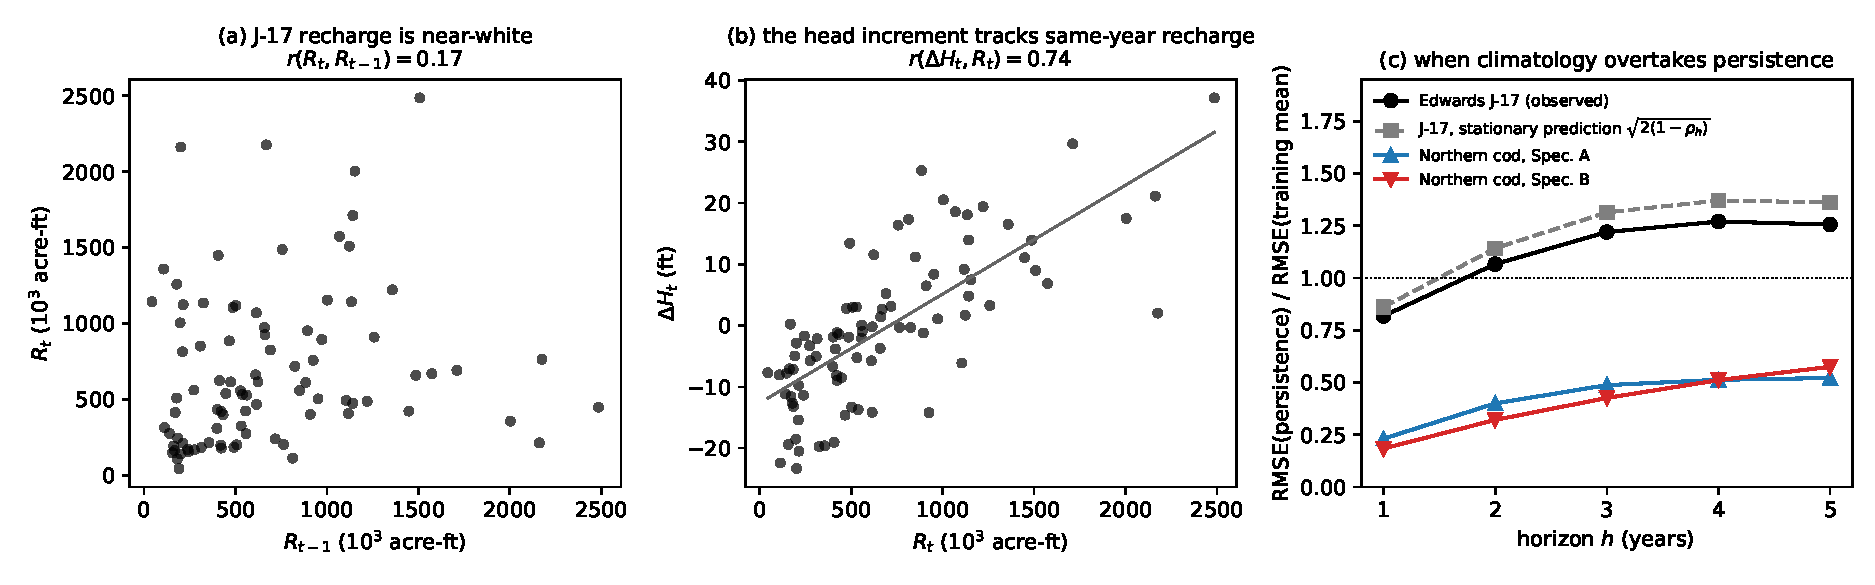
\includegraphics[width=\textwidth]{fig7_mechanism}
\caption{The two mechanisms behind the cross-system result. (a) J-17 annual recharge is near-white: $R_t$ against $R_{t-1}$, $r=0.17$. (b) The J-17 head increment tracks same-year recharge: $\Delta H_t$ against $R_t$, $r=0.74$; a balance that persists $R_t$ therefore substitutes a nearly uninformative value for the quantity that explains the increment (Proposition~\ref{prop:increment}(ii)). (c) Ratio of rolling-origin persistence RMSE to training-mean RMSE by horizon on the scored origin sets: J-17 observed (black) against the stationary prediction $\sqrt{2(1-\rho_h)}$ of Remark~\ref{rem:crossover} (grey, dashed), with the crossover at $h=2$; Northern cod Specifications A and B never cross within five years, and the stationary prediction does not apply to them.}
\label{fig:mechanism}
\end{figure}

\subsection{What transfers and what does not}\label{sec:transfer}

Table~\ref{tab:cross} sets the two systems side by side without pooling them. What transfers is the test and the reading of its outcome: a process-based increment forecaster must be scored against persistence and against its own next-simpler rung, on the predictand management uses, at the horizons advice uses, under a protocol stated in advance and disclosed where it was completed late; and when it fails, equation~\eqref{eq:decomp} says where to look, at the driver's predictability from the origin or at the mechanism's residual on the transitions that carry the error. What also transfers is the positive content of each failure. On J-17, the map nowcasts, so the operational question is how to obtain a recharge forecast, and the answer within the information set is that nothing available on 31 December supplies one, which directs effort toward within-year updating rather than toward the balance. On cod, the catch-supplied modules carry a short-memory growth term with one-step skill in a low-biomass regime on one specification, which is a testable claim for a prospective design, and the autonomous modules are refuted with high power, which retires one class of argument about this stock. What does not transfer is any number. The verdicts, margins, autocorrelations and power figures belong to their series, and a reader whose system has a more persistent driver than J-17's recharge, or a predictand that is stationary where cod is not, should expect a different verdict and should re-score rather than inherit one.

\begin{table}[!htb]
\centering\small
\caption{The two systems side by side. Nothing in this table is pooled; each column is one series under its own protocol. ``Failing term'' refers to equation~\eqref{eq:decomp}.}
\label{tab:cross}
\begin{tabularx}{\textwidth}{@{}>{\raggedright\arraybackslash}p{0.21\textwidth}LL@{}}
\toprule
 & Northern cod (Spec.\ A; Spec.\ B) & Edwards J-17 \\
\midrule
Predictand & assessed SSB, kt; retrospective vintage & measured annual-mean head, ft \\
Structural claim & surplus production; catch-driven stock flow; depensation; residual memory & one-pool water balance; residual and delay variants; climate-informed recharge \\
Driver at the origin & catch supplied (M2--M4) or held at training mean (M1, M1b) & recharge and pumpage persisted (M2), climatological (M2m), forecast from climate indices, or realised (oracle) \\
Protocol & C: 5\% band, both horizons, comparator and persistence & E: point rule at $h=1$, persistence and next-simpler causal model \\
One-year persistence RMSE & 98.0; 84.4\,kt & 13.23\,ft \\
Best structural module at $h=1$ & M1b 114.8 (ratio 1.17); M1 119.5 (1.42) & M2m 12.28 (declined by class clause); M1 12.84 (retained) \\
Retained & none; none & AR(1) under E (margin within noise); none under C \\
Failing term & misspecification: collapse transitions outside the class; floor forecasts after 1992 & substitution: $\rho(R)=0.17<\tfrac12$; the map nowcasts at 7.55\,ft \\
Lag-one autocorrelation of the mechanism & apparent net production 0.75; 0.91 & flux mechanism 0.08; recharge 0.17 \\
Baseline crossover (Remark~\ref{rem:crossover}) & none within five years; stationary formula inapplicable & at $h=2$, as predicted \\
What the test could see & power 97--99\% for a true M1; 9--11\% for a true M2; specificity 97--99\% in class & oracle 7.55\,ft, 43\% below persistence; climate indices add $\le0.13$\,ft \\
\bottomrule
\end{tabularx}
\end{table}
\FloatBarrier
\section{Related work and what is new}\label{sec:related}

\paragraph{Forecast evaluation.} Comparing the out-of-sample accuracy of competing forecasters on the same realisations, rather than their in-sample fit, is the established discipline for the question asked here \citep{Diebold1995,HyndmanKoehler2006,HyndmanAthanasopoulos2021}, and rolling-origin evaluation is its standard form for time series \citep{Tashman2000,Bergmeir2012}. The hazard that discipline guards against is selection after the fact: when many candidates are scored on one realisation, the best observed score is an upward-biased estimate of skill and per-comparison tests do not restore validity. White's reality check constructs the distribution of the best statistic across candidates under the null that none has skill \citep{White2000}, and stepwise procedures formalise the correction with control of the familywise error rate \citep{RomanoWolf2005}. The present design addresses the same hazard by a more restrictive and less general route, and the difference should be stated. Those procedures take a set of already-computed scores and ask which survive correction for having been selected. Here the model class, the baselines and the scoring core were fixed before scoring, each module must beat its own next-simpler rung and not only the field, and the retention predicate is then applied once; the completions made after scores were seen are disclosed, and the operating characteristics are estimated by simulation conditional on the rule as applied. That is not a familywise-error correction and is not presented as one.

\paragraph{Simple benchmarks are hard to beat.} That naive and simple statistical methods are close to the most accurate, and that sophisticated methods frequently fail to beat them, is the most consistently replicated result in forecasting: it organises the M3 and M4 competitions \citep{Makridakis2000,Makridakis2018}, in the latter of which none of the pure machine-learning entries was more accurate than the combination benchmark, and it has been found on fish population series \citep{Ward2014} and on simulated ecological dynamics \citep{Perretti2013}. The two results here are single-system instances of that phenomenon, and the scope difference is material: the competitions aggregate over tens of thousands of series and dozens of methods, whereas this paper scores two ladders on two systems. A cross-series result about method classes entails nothing about a particular stock or basin, and a two-system result does not generalise to method classes. What the two kinds of result share is the test, and what this paper adds to the phenomenon is a reason, in equation~\eqref{eq:decomp}, why a mechanistic increment forecaster loses to persistence when it does.

\paragraph{Fisheries.} Structural claims in stock assessment are usually examined through fit, retrospective pattern and simulation self-consistency \citep{HilbornWalters1992,Punt2016,Maunder2015}; where prediction skill is examined directly, it is computed on the fitted survey or catch-rate index through hindcast cross-validation \citep{Kell2016,Kell2021,Carvalho2021,Kokkalis2024}, while advice concerns the state, and the difficulties of fitting surplus-production models to series with little contrast are long documented \citep{HilbornWalters1992,LudwigWalters1985,Polacheck1993,Punt2003,PedersenBerg2017}. The Northern cod collapse and its non-recovery have an extensive literature establishing the empirical facts \citep{Hutchings1994,Myers1997,Walters1996,Hutchings2005,RoseRowe2015,RoseWalters2019,Rose2026} and debating depensation \citep{Shelton1999,Hutchings1996,Myers1995,Liermann1997}. This paper's contribution to that literature is different in kind: it measures what those facts do to the forecast skill of a familiar model class from fixed origins, locates the deficit in the collapse transitions, proves that those transitions lie outside the class at the recorded catch, and reports the power of the test. It is a conditional hindcast, scored against a retrospective vintage with catch supplied along the horizon; it is not an operational forecast evaluation and licenses no claim about the performance of the assessment process as it ran.

\paragraph{Groundwater.} Groundwater-level forecasting at index wells is a mature area with statistical, neural-network and process-based approaches on annual and sub-annual series \citep{Daliakopoulos2005,AdamowskiChan2011}, and it has begun to institutionalise benchmark culture: GEMS-GER standardises 32 years of weekly observations from 3\,207 German wells with three benchmark models of increasing complexity \citep{Ohmer2026}, and a systematic comparison of nine machine-learning architectures on a karst catchment finds that aquifer complexity rather than algorithm choice bounds predictability \citep{Zhu2026}. Those studies compare model families against one another. None subjects a deliberately simple process-based water balance to a scored ablation against persistence and the training mean under a rule fixed in advance, and none reports a training mean beating persistence at a multi-year horizon on this basin. On the Edwards Aquifer, regional flow has long been represented, and debated, through equivalent-porous-media and lumped approaches \citep{Scanlon2003}; the one-pool map is not a karst model and the lumped-versus-distributed question is inherited rather than settled here. The climate predictors enter because ENSO phases shift North American precipitation \citep{Ropelewski1986}, and the finding that they add at most 0.13\,ft at the annual origin is a statement about this information set, not about ENSO.

\paragraph{What is new.} Relative to the two single-system studies and their earlier two-part combination, this article contributes (a) one scored test reported on two systems under two disclosed protocols without pooling, with the aquifer verdict stated under both; (b) Proposition~\ref{prop:increment}, which decomposes the one-step skill of any increment forecaster into a substitution term governed by the driver's lag-one autocorrelation and a misspecification term governed by the mechanism's residual, with the half-autocorrelation threshold and the never-loses property of climatological drivers as corollaries; (c) Remark~\ref{rem:crossover}, the half-autocorrelation crossover of the two baselines, verified on J-17 at every horizon and shown to fail, informatively, on the non-stationary cod series; (d) the correction of the earlier cross-system reading, which attributed the cod failure to a weakly autocorrelated driver; and (e) for the cod half, the period decomposition, the identification result and the operating characteristics that the single-system article introduced, now placed beside the aquifer's oracle diagnostic as two answers to the same question of what the test could see.
\FloatBarrier
\section{Discussion}\label{sec:discussion}

\subsection{Why a negative result is informative here}\label{sec:whyinformative}

A finding that a model family fails is worth little unless three things are true of the test: that the rule was fixed before the scores were seen, that the test had the power to find the structure had it been there, and that the failure can be located. The first holds in the qualified form stated in Section~\ref{sec:protocols}: the scoring cores were coded before the first pass of each system, the later completions are disclosed, and none of them decides a verdict. The second is established by different instruments in the two systems, simulation under known truth on cod (power 97--99\% against the autonomous module, 9--11\% against the stock-flow module, so the verdict is strong against one and weak against the other) and the oracle on J-17 (the map nowcasts at 7.55\,ft, so the mechanism is capable of explaining the increment). The third is what Proposition~\ref{prop:increment} supplies: the cod deficit is a misspecification term concentrated in the 1991--1995 transitions, which no member of the class can produce at the recorded catch (Proposition~\ref{prop:repeller}), and the J-17 deficit is a substitution term, the variance of a flux mechanism whose lag-one autocorrelation is 0.08 persisted as if it were one. Located failures tell the modeller where to look next. On the aquifer it is within-year information: the gap between persistence and the oracle is next year's recharge, nothing available on 31 December forecasts it, and the operational question becomes at what point in the year a nowcast with partial-year fluxes beats the annual persistence forecast, which is a new evaluation protocol rather than a new module. On the stock it is the regime: the catch-supplied modules carry a short-memory growth term with one-step skill in a low-biomass regime on one specification, and a prospective test of that claim would fix the regime boundary from a criterion external to the scores, use the consistent catch-timing convention, apply the band at both horizons and require the result on both series.

\subsection{Protocols, bands and the AR(1)}\label{sec:protocoldiff}

The two protocols disagree about exactly one module, and the disagreement is instructive rather than embarrassing. Under the aquifer's point rule the AR(1) is retained by 0.39\,ft; under the cod rule's 5\% band and two-horizon requirement it is not, because 2.96\% is inside the band and the five-year ordering reverses. The uncertainty layer sides with the stricter rule in the sense that matters: the margin's interval covers zero in both bootstrap implementations, MAE is a tie, and the five-year loss is real. The simulation on cod says what the band buys in general, most of the rule's specificity for a small cost in power (SI S8), and the AR(1) case says what it buys in particular: protection against retaining a one-horizon, within-noise margin. We therefore report the AR(1) as retained under Protocol E, as the frozen rule requires, and as a weak-autocorrelation phenomenon with no transferable content, as the evidence requires. The complementary protocol lesson comes from M2m. The best one-step forecaster on J-17 was declined by a class clause outside the retention predicate; the clause was recorded in the frozen documents, but on the rule as written M2m passes, and its margin over persistence is the only one-year margin on the series that separates from noise. A protocol that can decline the best forecaster by a clause outside its predicate should say so in its verdict, and the verdict here does: no stock-flow module is retained, and the statement is an artefact of the clause rather than of the scores.

\subsection{Limitations}\label{sec:limits}

The test is on two systems, three series, two model classes and two horizons; it is a demonstration and a replication, not a survey. On cod, each specification uses a single retrospective vintage, which favours the models (the 1983--2015 overlap between vintages differs by 24.7\,kt on average and by 131\,kt in one year), catch enters as a point series although both assessments treat it as bounded and the collapse years are under-reported, the forecasts are point forecasts scored by RMSE and MAE rather than predictive distributions scored by proper rules, sample sizes are small on Specification A, the period bands were chosen after seeing the data, the archived runner's catch-timing offset moves the catch-supplied modules' one-step margins by 20--75\,kt without moving the verdict, and the operating characteristics were measured against truths inside the class and two specific truths outside it. On J-17, total-area recharge and pumpage mix the San Antonio and Uvalde pools, recharge is a stream-loss estimate, pumpage includes unreported domestic, livestock and federal use, next-year pumpage is partly an institutional response to head rather than an exogenous flux, the map is not a karst model and the lumped-versus-distributed question is inherited, the sample is 90 years with four short fixed windows, and the nClimDiv precipitation file is not redistributed, so the three precipitation columns of the registered panel are reproducible from the provenance URL rather than from the archive alone. Proposition~\ref{prop:increment} is exact but its application is stylised: the J-17 numbers in Section~\ref{sec:decomp} use full-sample rather than rolling parameters, treat the drain term as common to both forecasters, and require the orthogonality $\E[u_{t+1}m_t]=0$, which holds approximately for a mechanism whose residual is the next year's recharge surprise but is an assumption nonetheless. Remark~\ref{rem:crossover} requires stationarity, which J-17 satisfies approximately and cod does not; its failure on cod is reported as a failure. Neither protocol was prospectively registered, and nothing in this paper should be read as a claim that it was.

\section{Conclusions}\label{sec:conclusions}

Scored on the predictand that management uses, against last-value persistence and the training mean, under protocols whose scoring cores were fixed before the first pass and whose later completions are disclosed, no structural module of a surplus-production ladder is retained on the spawning-stock biomass of Northern cod on either of two assessment series, and no structural module of a one-pool water-balance ladder is retained on the annual-mean head of the Edwards Aquifer at J-17, where the one module the aquifer's point rule retains is a univariate AR(1) with a margin inside the noise. The cod modules fail because the collapse that carries the error lies outside the model class at the recorded catch and because training-mean catch drives the autonomous modules to the floor after it; the aquifer modules fail because annual recharge is near-white and a balance that persists it substitutes an uninformative value for the quantity that explains the increment, while the same balance given the year's fluxes nowcasts at 7.55\,ft. These are the two terms of one decomposition: a one-step increment forecaster gains on persistence only through what its mechanism fits of the realised increment and loses whatever its substituted driver fails to persist, the latter term being negative whenever the driver's lag-one autocorrelation is below one half and zero when the driver is replaced by its mean; and the training mean overtakes persistence at the horizon at which the predictand's autocorrelation falls below one half, which on J-17 is two years and on the non-stationary cod series never within five. The implication for practice is procedural and general even where the numbers are not. Claims that a structural element improves prediction should be made on the state, against persistence and the next-simpler model, at the horizons advice uses, under a rule declared in advance, accompanied by what the test could have seen, and, when they fail, located in the mechanism or in the driver so that the next model is built where the error is. Mechanistic fidelity is a hypothesis about accuracy. In two unrelated systems it was scored, and in both it failed for a reason that can be stated.
\appendix
\FloatBarrier
\section{Proofs}\label{app:proofs}

\paragraph{Proof of Proposition~\ref{prop:repeller}.} Throughout, $F_C(S) = \max(S + g(S) - C,\,0)$; the numerical floor $\epsilon = 10^{-3}\kt$ used in the computations replaces $0$ by $\epsilon$ and changes nothing below.

\emph{(i)} Let $0 \le S < S_-(C)$. If $g(S) \ge C$ then $S$ belongs to the set $\{S'>0 : g(S')\ge C\}$ (for $S>0$) or $g(0)=0\ge C>0$ (for $S=0$), both impossible; hence $g(S) < C$ and $S + g(S) - C < S$. Therefore $0 \le F_C(S) \le \max(S,0) = S < S_-(C)$. By induction a trajectory started in $[0,S_-(C))$ is nonincreasing and never leaves the interval. If $g(S) \ge C$ on an interval $I$ and $S\in I$, then $S + g(S) - C \ge S \ge 0$, so $F_C(S) = S + g(S) - C \ge S$.

\emph{(ii)} Suppose $S_{t+1} = F_{C_t}(S_t) < S_t - C_t$. If the maximum in $F_{C_t}$ is attained by the first argument, $S_t + g(S_t) - C_t < S_t - C_t$ gives $g(S_t) < 0$. If it is attained by $0$, then $S_t + g(S_t) - C_t \le 0 < S_t - C_t$ (the right inequality because $S_{t+1} = 0 < S_t - C_t$), and again $g(S_t) < 0$. On the compensatory branch $g(S) = rS(1-S/K) \ge 0$ for $0 \le S \le K$. On the depensatory branch $g(S) = rS(1-S/K)(S-\sA)/(K-\sA)$ with $0<\sA<K$, which for $0<S<K$ is negative exactly when $S<\sA$. \qed

For the Schaefer branch the equation $g(S)=C$ has the roots $S_\pm(C) = \tfrac{K}{2}\bigl(1\pm\sqrt{1-4C/(rK)}\bigr)$ when $4C\le rK$, $g\ge C$ on $[S_-,S_+]$ and $g<C$ outside, so $S_-(C)$ in the proposition is the lower root and $[S_-(C),S_+(C)]$ the interval on which the autonomous map cannot decline. $F_C'(S_+) = 1 + g'(S_+) = 1 + r(1-2S_+/K)$, which at the collapse-window fit under $C=240\kt$ equals $-0.39$.

\paragraph{Proof of Proposition~\ref{prop:increment}.} The forecast error of $\hat y$ is $\Delta_{t+1}-m(\hat x_{t+1}) = (m_{t+1}-m(\hat x_{t+1})) + (\Delta_{t+1}-m_{t+1}) = d_{t+1}+u_{t+1}$, and the error of persistence is $\Delta_{t+1} = m_{t+1}+u_{t+1}$. Hence
\begin{align*}
\MSE(\hat y)-\MSE(\pers) &= \E[d^2]+2\E[du]+\E[u^2] - \E[m^2]-2\E[mu]-\E[u^2]\\
&= \E[d^2]-\E[m^2] + 2\E\bigl[u\,(d-m_{t+1})\bigr],
\end{align*}
and $d-m_{t+1} = -m(\hat x_{t+1})$, which is \eqref{eq:decomp}.

\emph{(i)} With $\hat x_{t+1}=x_{t+1}$, $d\equiv 0$ and \eqref{eq:decomp} reads $-\E[m^2]-2\E[um] = \E[u^2]-\E[(u+m)^2] = \E[u^2]-\E[\Delta^2]$.

\emph{(ii)} With $\hat x_{t+1}=x_t$, $d_{t+1}=m_{t+1}-m_t$, and weak stationarity gives $\E[d^2] = 2\sigma^2 - 2\operatorname{cov}(m_{t+1},m_t) = 2\sigma^2(1-\rho)$ and $\E[m^2]=\sigma^2+\mu^2$. The misspecification term is $-2\E[u_{t+1}m_t]=0$ by hypothesis. Hence $\MSE(\hat y)-\MSE(\pers) = 2\sigma^2(1-\rho)-\sigma^2-\mu^2 = \sigma^2(1-2\rho)-\mu^2$, which is negative if and only if $\rho > \tfrac12 - \mu^2/(2\sigma^2)$.

\emph{(iii)} With $m(\hat x_{t+1})=\mu$, $d_{t+1}=m_{t+1}-\mu$, $\E[d^2]=\sigma^2$, and the misspecification term is $-2\mu\E[u]=0$. Hence $\MSE(\hat y)-\MSE(\pers) = \sigma^2-(\sigma^2+\mu^2) = -\mu^2$. Subtracting the expression in (ii) gives $\MSE(\text{climatological})-\MSE(\text{persisted}) = -\mu^2 - \sigma^2(1-2\rho)+\mu^2 = -\sigma^2(1-2\rho)$. \qed

\paragraph{Derivation of Remark~\ref{rem:crossover}.} For weakly stationary $y$ with mean $\bar y$, variance $\sigma_y^2$ and lag-$h$ autocorrelation $\rho_h$, the $h$-step persistence error is $y_{t+h}-y_t$ with mean zero and variance $2\sigma_y^2(1-\rho_h)$, and the error of the known-mean forecast is $y_{t+h}-\bar y$ with mean square $\sigma_y^2$. The ratio of root mean squared errors is therefore $\sqrt{2(1-\rho_h)}$, which is below one if and only if $\rho_h>\tfrac12$. With the mean estimated from $n_t$ training values, $\MSE_h(\mathrm{mean}) = \sigma_y^2 + \operatorname{Var}(\hat{\bar y}_t) - 2\operatorname{cov}(y_{t+h},\hat{\bar y}_t)$, whose correction terms are of order $\sigma_y^2/n_t$ times sums of autocorrelations and vanish as $n_t\to\infty$. \qed

\section*{Declarations}

\paragraph{Lineage} This article unifies two single-system studies, a scored surplus-production ladder on Northern cod \citep{Abaee2026cod} and a scored one-pool water-balance ladder on Edwards Aquifer head \citep{Abaee2026edwards}, whose archived scores it reports unchanged, and it supersedes their earlier two-part combination. The two systems are reported under their own protocols and are not pooled.

\paragraph{Data availability} All input data, analysis scripts, result files and the frozen protocol documents of both systems are archived at \url{https://github.com/MIKEAA2020/general-sustainability}, with Zenodo records for the cod study (\url{https://zenodo.org/records/22553609}) and the aquifer study (\url{https://doi.org/10.5281/zenodo.22552680}). Cod: the NCAM Table A2 and xteNCAM Table 17 files, the landings tables, the capelin acoustic index and the RAM Legacy Stock Assessment Database v4.66 extract (10.5281/zenodo.14043038; stock COD2J3KL) are archived in-repository under \texttt{paperE1\_calibration\_data\_v1\_wave\_e\_cod/} and \texttt{wave\_e\_cod/data/} with their source record. Aquifer: J-17 daily highs are Texas Water Development Board well 6837203; recharge is the USGS data release of \citet{UmphresChoi2025}; pumpage is Edwards Aquifer Authority Table 1 \citep{EAA2024}; Comal Springs discharge is USGS 08168710; Ni\~no~3.4 is NOAA PSL HadISST (raw file registered); precipitation is NCEI nClimDiv, whose raw file is not redistributed (provenance URL archived), so the three precipitation columns of the registered twenty-column panel \texttt{wave\_e\_edwards/data/annual\_panel.csv} rebuild from the provenance source rather than from the archive alone, while scoring from the registered panel does not require it.

\paragraph{Code availability} The cod ladder and its campaigns are produced by \texttt{wave\_e\_cod/src/run\_ladder.py}, \texttt{run\_xte.py}, \texttt{run\_capelin\_regime.py}, \texttt{run\_capelin\_index.py}, the uncertainty script \texttt{campaign\_e1\_dm\_uncertainty\_regime.py} and the simulation \texttt{sim\_retention\_power.py}, with the paired bootstrap, period decomposition, catch-timing sensitivity and figure scripts archived under the previous edition's \texttt{work/} directory and carried in \texttt{paper11\_forecasting\_baselines\_v67\_src/work/}. The aquifer ladder is produced by \texttt{wave\_e\_edwards/src/run\_ladder.py}, the climate pass by \texttt{run\_recharge.py}, the uncertainty layer by \texttt{e3\_audit\_uncertainty.py} with its independent replication \texttt{campaign\_e3\_dm\_uncertainty.py}, and the pumpage counterfactuals by \texttt{campaign\_e3\_pumpage\_scenarios.py}; the verification script \texttt{paperE3\_edwards\_forecast\_ladder\_v17\_verification.py} re-runs the ladder from the registered panel and recompares every results-table cell. The computations new to this edition, the horizon profile of the two baselines on all three series, the autocorrelations of Section~\ref{sec:synthesis} and Fig.~\ref{fig:mechanism}, are produced by \texttt{work/horizon\_profile.py} and \texttt{work/make\_fig\_mechanism.py} in the source directory from the registered data files alone; their outputs are tabulated in SI S23, and the $h=1$ and $h=5$ baseline values they regenerate agree with the archived summaries to the printed precision. The verification script \texttt{paper11\_forecasting\_baselines\_v67\_verification.py} asserts every number quoted in the main text from the archived result files and the registered data.

\paragraph{Reproducibility} All computations are deterministic within a fixed interpreter and library stack. The cod runners were re-executed in a third software environment for the previous edition and every scored row reproduced at printed precision, with one known environment sensitivity (the M1b optimum on Specification B, $\pm17\kt$, immaterial to the verdict; SI S13). The aquifer scripts regenerate every archived result file byte for byte in a fresh environment, and the two implementations of the uncertainty layer agree on every conclusion under different seeds, block lengths and HAC conventions (SI S18).

\paragraph{CRediT authorship contribution statement} Amin Abaee: Conceptualization, Methodology, Software, Validation, Formal analysis, Investigation, Data curation, Writing -- original draft, Writing -- review \& editing, Visualization.

\paragraph{Funding} This research did not receive any specific grant from funding agencies in the public, commercial, or not-for-profit sectors.

\paragraph{Declaration of competing interest} The author declares no known competing financial interests or personal relationships that could have appeared to influence the work reported in this paper.

\paragraph{Declaration of generative AI in the writing process} GLM (Z.ai), Qwen (Alibaba Cloud) and DeepSeek AI assisted with drafting and iterative review. The author reviewed and edited all outputs and takes full responsibility for the final work.

\begin{thebibliography}{99}
\providecommand{\natexlab}[1]{#1}

\bibitem[Abaee(2026a)]{Abaee2026edwards}
Abaee, A., 2026a. Does a one-pool water-balance model improve forecasts of Edwards Aquifer head? A scored test at J-17. Zenodo. \url{https://doi.org/10.5281/zenodo.22552680}

\bibitem[Abaee(2026b)]{Abaee2026cod}
Abaee, A., 2026b. Does a surplus-production ladder improve forecasts of Northern cod? A scored retention test against persistence on NAFO 2J3KL. Zenodo. \url{https://zenodo.org/records/22553609}

\bibitem[Adamowski and Chan(2011)]{AdamowskiChan2011}
Adamowski, J., Chan, H.F., 2011. A wavelet neural network conjunction model for groundwater level forecasting. J. Hydrol. 407, 28--40. \url{https://doi.org/10.1016/j.jhydrol.2011.06.013}

\bibitem[Bergmeir and Ben{\'\i}tez(2012)]{Bergmeir2012}
Bergmeir, C., Ben{\'\i}tez, J.M., 2012. On the use of cross-validation for time series predictor evaluation. Inf. Sci. 191, 192--213.

\bibitem[Buren et al.(2014)]{Buren2014}
Buren, A.D., Koen-Alonso, M., Pepin, P., Mowbray, F., Nakashima, B., Stenson, G., Ollerhead, N., Montevecchi, W.A., 2014. Bottom-up regulation of capelin, a keystone forage species. PLoS ONE 9, e87589.

\bibitem[Cadigan(2016)]{Cadigan2016}
Cadigan, N.G., 2016. A state-space stock assessment model for northern cod, including under-reported catches and variable natural mortality rates. Can. J. Fish. Aquat. Sci. 73, 296--308.

\bibitem[Carvalho et al.(2021)]{Carvalho2021}
Carvalho, F., Winker, H., Courtney, D., Kapur, M., Kell, L., Cardinale, M., Schirripa, M., Kitakado, T., Yemane, D., Piner, K.R., Maunder, M.N., Taylor, I., Wetzel, C.R., Doering, K., Johnson, K.F., Methot, R.D., 2021. A cookbook for using model diagnostics in integrated stock assessments. Fish. Res. 240, 105959.

\bibitem[Daliakopoulos et al.(2005)]{Daliakopoulos2005}
Daliakopoulos, I.N., Coulibaly, P., Tsanis, I.K., 2005. Groundwater level forecasting using artificial neural networks. J. Hydrol. 309, 229--240. \url{https://doi.org/10.1016/j.jhydrol.2004.12.001}

\bibitem[DFO(2009)]{DFO2009}
DFO, 2009. A fishery decision-making framework incorporating the Precautionary Approach. Fisheries and Oceans Canada, Ottawa.

\bibitem[DFO(2016)]{DFO2016}
DFO, 2016. Stock assessment of Northern cod (NAFO Divs. 2J3KL) in 2016. DFO Can. Sci. Advis. Sec. Sci. Advis. Rep. 2016/026.

\bibitem[DFO(2024a)]{DFO2024a}
DFO, 2024a. NAFO Divisions 2J3KL Northern Cod stock assessment to 2024. DFO Can. Sci. Advis. Sec. Sci. Advis. Rep. 2024/049.

\bibitem[DFO(2024b)]{DFO2024b}
DFO, 2024b. Assessment of capelin in NAFO Divisions 2J3KL. DFO Can. Sci. Advis. Sec. Sci. Advis. Rep. 2024/050.

\bibitem[Diebold and Mariano(1995)]{Diebold1995}
Diebold, F.X., Mariano, R.S., 1995. Comparing predictive accuracy. J. Bus. Econ. Stat. 13, 253--263.

\bibitem[Diebold(2015)]{Diebold2015}
Diebold, F.X., 2015. Comparing predictive accuracy, twenty years later: a personal perspective on the use and abuse of Diebold--Mariano tests. J. Bus. Econ. Stat. 33, 1--9.

\bibitem[Edwards Aquifer Authority(2024)]{EAA2024}
Edwards Aquifer Authority, 2024. 2023 Groundwater Discharge and Usage, Table 1 (after USGS letter report, 5 April 2024). Edwards Aquifer Authority, San Antonio, TX. \url{https://www.edwardsaquifer.org/wp-content/uploads/2025/05/2023-Groundwater-Discharge-and-Usage.pdf}

\bibitem[Harvey et al.(1997)]{Harvey1997}
Harvey, D., Leybourne, S., Newbold, P., 1997. Testing the equality of prediction mean squared errors. Int. J. Forecast. 13, 281--291.

\bibitem[Hilborn and Walters(1992)]{HilbornWalters1992}
Hilborn, R., Walters, C.J., 1992. Quantitative Fisheries Stock Assessment: Choice, Dynamics and Uncertainty. Chapman and Hall, New York.

\bibitem[Hutchings and Myers(1994)]{Hutchings1994}
Hutchings, J.A., Myers, R.A., 1994. What can be learned from the collapse of a renewable resource? Atlantic cod, \emph{Gadus morhua}, of Newfoundland and Labrador. Can. J. Fish. Aquat. Sci. 51, 2126--2146.

\bibitem[Hutchings(1996)]{Hutchings1996}
Hutchings, J.A., 1996. Spatial and temporal variation in the density of northern cod and a review of hypotheses for the stock's collapse. Can. J. Fish. Aquat. Sci. 53, 943--962.

\bibitem[Hutchings(2005)]{Hutchings2005}
Hutchings, J.A., 2005. Life history consequences of overexploitation to population recovery in Northwest Atlantic cod (\emph{Gadus morhua}). Can. J. Fish. Aquat. Sci. 62, 824--832.

\bibitem[Hyndman and Athanasopoulos(2021)]{HyndmanAthanasopoulos2021}
Hyndman, R.J., Athanasopoulos, G., 2021. Forecasting: Principles and Practice, third ed. OTexts, Melbourne.

\bibitem[Hyndman and Koehler(2006)]{HyndmanKoehler2006}
Hyndman, R.J., Koehler, A.B., 2006. Another look at measures of forecast accuracy. Int. J. Forecast. 22, 679--688.

\bibitem[Kell et al.(2016)]{Kell2016}
Kell, L.T., Kimoto, A., Kitakado, T., 2016. Evaluation of the prediction skill of stock assessment using hindcasting. Fish. Res. 183, 119--127.

\bibitem[Kell et al.(2021)]{Kell2021}
Kell, L.T., Sharma, R., Kitakado, T., Winker, H., Mosqueira, I., Cardinale, M., Fu, D., 2021. Validation of stock assessment methods: is it me or my model talking? ICES J. Mar. Sci. 78, 2244--2255.

\bibitem[Kokkalis et al.(2024)]{Kokkalis2024}
Kokkalis, A., Berg, C.W., Kapur, M.S., Winker, H., Jacobsen, N.S., Taylor, M.H., Ichinokawa, M., Miyagawa, M., Medeiros-Leal, W., Nielsen, J.R., Mildenberger, T.K., 2024. Good practices for surplus production models. Fish. Res. 275, 107010.

\bibitem[K{\"u}nsch(1989)]{Kunsch1989}
K{\"u}nsch, H.R., 1989. The jackknife and the bootstrap for general stationary observations. Ann. Stat. 17, 1217--1241.

\bibitem[Liermann and Hilborn(1997)]{Liermann1997}
Liermann, M., Hilborn, R., 1997. Depensation in fish stocks: a hierarchic Bayesian meta-analysis. Can. J. Fish. Aquat. Sci. 54, 1976--1984.

\bibitem[Ludwig and Walters(1985)]{LudwigWalters1985}
Ludwig, D., Walters, C.J., 1985. Are age-structured models appropriate for catch-effort data? Can. J. Fish. Aquat. Sci. 42, 1066--1072.

\bibitem[Makridakis and Hibon(2000)]{Makridakis2000}
Makridakis, S., Hibon, M., 2000. The M3-Competition: results, conclusions and implications. Int. J. Forecast. 16, 451--476.

\bibitem[Makridakis et al.(2018)]{Makridakis2018}
Makridakis, S., Spiliotis, E., Assimakopoulos, V., 2018. The M4 Competition: results, findings, conclusion and way forward. Int. J. Forecast. 34, 802--808.

\bibitem[Maunder and Piner(2015)]{Maunder2015}
Maunder, M.N., Piner, K.R., 2015. Contemporary fisheries stock assessment: many issues still remain. ICES J. Mar. Sci. 72, 7--18.

\bibitem[Murphy et al.(2025)]{Murphy2025}
Murphy, H.M., Adamack, A.T., Lewis, R.S., Bourne, C.M., 2025. Assessment of capelin in NAFO Divisions 2J+3KL to 2023. DFO Can. Sci. Advis. Sec. Res. Doc. 2025/022.

\bibitem[Myers et al.(1995)]{Myers1995}
Myers, R.A., Barrowman, N.J., Hutchings, J.A., Rosenberg, A.A., 1995. Population dynamics of exploited fish stocks at low population levels. Science 269, 1106--1108.

\bibitem[Myers et al.(1997)]{Myers1997}
Myers, R.A., Hutchings, J.A., Barrowman, N.J., 1997. Why do fish stocks collapse? The example of cod in Atlantic Canada. Ecol. Appl. 7, 91--106.

\bibitem[Northwest Atlantic Fisheries Centre(2025)]{NAFC2025}
Northwest Atlantic Fisheries Centre, 2025. 2J3KL cod and capelin biomass indices. Zenodo. \url{https://doi.org/10.5281/zenodo.17515115}

\bibitem[Ohmer et al.(2026)]{Ohmer2026}
Ohmer, M., Liesch, T., Habbel, B., Heudorfer, B., Gomez, M., Clos, P., N{\"o}lscher, M., Broda, S., 2026. GEMS-GER: a machine learning benchmark dataset of long-term groundwater levels in Germany with meteorological forcings and site-specific environmental features. Earth Syst. Sci. Data 18, 77.

\bibitem[Pedersen and Berg(2017)]{PedersenBerg2017}
Pedersen, M.W., Berg, C.W., 2017. A stochastic surplus production model in continuous time. Fish Fish. 18, 226--243.

\bibitem[Pella and Tomlinson(1969)]{Pella1969}
Pella, J.J., Tomlinson, P.K., 1969. A generalized stock production model. Bull. Inter-Am. Trop. Tuna Comm. 13, 419--496.

\bibitem[Perretti et al.(2013)]{Perretti2013}
Perretti, C.T., Munch, S.B., Sugihara, G., 2013. Model-free forecasting outperforms the correct mechanistic model for simulated and experimental data. Proc. Natl. Acad. Sci. U.S.A. 110, 5253--5257.

\bibitem[Polacheck et al.(1993)]{Polacheck1993}
Polacheck, T., Hilborn, R., Punt, A.E., 1993. Fitting surplus production models: comparing methods and measuring uncertainty. Can. J. Fish. Aquat. Sci. 50, 2597--2607.

\bibitem[Puente(1978)]{Puente1978}
Puente, C., 1978. Method of estimating natural recharge to the Edwards Aquifer in the San Antonio area, Texas. U.S. Geological Survey Water-Resources Investigations Report 78-10, Austin, TX.

\bibitem[Punt et al.(2016)]{Punt2016}
Punt, A.E., Butterworth, D.S., de Moor, C.L., De Oliveira, J.A.A., Haddon, M., 2016. Management strategy evaluation: best practices. Fish Fish. 17, 303--334.

\bibitem[Punt(2003)]{Punt2003}
Punt, A.E., 2003. Extending production models to include process error in the population dynamics. Can. J. Fish. Aquat. Sci. 60, 1217--1228.

\bibitem[Regular et al.(2025)]{Regular2025}
Regular, P.M., et al., 2025. Assessment of the Northern Cod stock in NAFO Divisions 2J3KL in 2024. DFO Can. Sci. Advis. Sec. Res. Doc. 2025/048.

\bibitem[Ricard et al.(2012)]{Ricard2012}
Ricard, D., Minto, C., Jensen, O.P., Baum, J.K., 2012. Examining the knowledge base and status of commercially exploited marine species with the RAM Legacy Stock Assessment Database. Fish Fish. 13, 380--398.

\bibitem[Romano and Wolf(2005)]{RomanoWolf2005}
Romano, J.P., Wolf, M., 2005. Stepwise multiple testing as formalized data snooping. Econometrica 73, 1237--1282.

\bibitem[Ropelewski and Halpert(1986)]{Ropelewski1986}
Ropelewski, C.F., Halpert, M.S., 1986. North American precipitation and temperature patterns associated with the El Ni{\~n}o/Southern Oscillation (ENSO). Mon. Weather Rev. 114, 2352--2362.

\bibitem[Rose and Rowe(2015)]{RoseRowe2015}
Rose, G.A., Rowe, S., 2015. Northern cod comeback. Can. J. Fish. Aquat. Sci. 72, 1789--1798.

\bibitem[Rose and Walters(2019)]{RoseWalters2019}
Rose, G.A., Walters, C.J., 2019. The state of Canada's iconic Northern cod: a second opinion. Fish. Res. 219, 105314.

\bibitem[Rose(2026)]{Rose2026}
Rose, G.A., 2026. Northern cod comeback: 10 years after. Can. J. Fish. Aquat. Sci. 83, 1--14. \url{https://doi.org/10.1139/cjfas-2025-0141}

\bibitem[Scanlon et al.(2003)]{Scanlon2003}
Scanlon, B.R., Mace, R.E., Barrett, M.E., Smith, B., 2003. Can we simulate regional groundwater flow in a karst system using equivalent porous media models? Case study, Barton Springs Edwards aquifer, USA. J. Hydrol. 276, 137--158.

\bibitem[Schaefer(1954)]{Schaefer1954}
Schaefer, M.B., 1954. Some aspects of the dynamics of populations important to the management of the commercial marine fisheries. Bull. Inter-Am. Trop. Tuna Comm. 1(2), 27--56.

\bibitem[Schijns et al.(2021)]{Schijns2021}
Schijns, R., Froese, R., Hutchings, J.A., Pauly, D., 2021. Five centuries of cod catches in Eastern Canada. ICES J. Mar. Sci. 78, 2675--2683.

\bibitem[Shelton and Healey(1999)]{Shelton1999}
Shelton, P.A., Healey, B.P., 1999. Should depensation be dismissed as a possible explanation for the lack of recovery of the northern cod (\emph{Gadus morhua}) stock? Can. J. Fish. Aquat. Sci. 56, 1521--1524.

\bibitem[Tashman(2000)]{Tashman2000}
Tashman, L.J., 2000. Out-of-sample tests of forecasting accuracy: an analysis and review. Int. J. Forecast. 16, 437--450.

\bibitem[Umphres and Choi(2025)]{UmphresChoi2025}
Umphres, G.D., Choi, N.J., 2025. Estimated annual recharge to the Edwards Aquifer in the San Antonio area, by stream basin or ungaged area, 1934--2024. U.S. Geological Survey data release. \url{https://doi.org/10.5066/P1BI62NY}

\bibitem[Walters and Maguire(1996)]{Walters1996}
Walters, C., Maguire, J.-J., 1996. Lessons for stock assessment from the northern cod collapse. Rev. Fish Biol. Fish. 6, 125--137.

\bibitem[Ward et al.(2014)]{Ward2014}
Ward, E.J., Holmes, E.E., Thorson, J.T., Collen, B., 2014. Complexity is costly: a meta-analysis of parametric and non-parametric methods for short-term population forecasting. Oikos 123, 652--661.

\bibitem[White(2000)]{White2000}
White, H., 2000. A reality check for data snooping. Econometrica 68, 1097--1126.

\bibitem[Zhu et al.(2026)]{Zhu2026}
Zhu, Q., Zhu, Y., Niu, J., Huang, J., Huang, F., Zhou, X., Liu, D., Hu, B.X., 2026. Benchmarking machine learning and deep learning models for groundwater level prediction in karst aquifers: the dominant role of hydrogeological complexity. Water 18, 939. \url{https://doi.org/10.3390/w18080939}

\end{thebibliography}

\end{document}
